

% Header mit Deklarationen
\documentclass[%
	pdftex,%              PDFTex verwenden
	a4paper,%             A4 Papier
	twoside,%             Einseitig/ wzeiseitig
	bibtotoc,%    		Literaturverzeichnis einfügen bibtotocnumbered: nummeriert
	liststotoc,%		Verzeichnisse einbinden in toc
	idxtotoc,%            Index ins Verzeichnis einfügen
	halfparskip,%        Europäischer Satz mit abstand zwischen Absätzen
	%chapterprefix,%       Kapitel anschreiben als Kapitel
	headsepline,%         Linie nach Kopfzeile
	footsepline,%         Linie vor Fusszeile
	pointlessnumbers,%     Nummern ohne abschließenden Punkt
	12pt,%                 Grössere Schrift, besser lesbar am bildschrim
	bibliography=totoc,
	cleardoublepage=empty,
	index=totoc,
	listof=totoc,
]{scrreprt}

%Maxi Biblio-Management
\usepackage[square,numbers]{natbib}
\bibliographystyle{unsrtdin}

%Zindath Biliothek Management
%\usepackage[backend=bibtex,bibencoding=ascii,style=numeric,citestyle=numeric-comp,defernumbers=true]{biblatex} 

%
% Seitenränder
%
\usepackage{geometry}
\geometry{a4paper, top=30mm, left=30mm, right=20mm, bottom=25mm, headsep=10mm, footskip=10mm}



%
% Paket für Übersetzungen ins Deutsche
%
\usepackage[french,english,ngerman]{babel}

%
% Pakete um Latin1 Zeichnensätze verwenden zu können und die dazu
% passenden Schriften.
%
%\usepackage[latin1]{inputenc}
% UTF8 Kompatabilität
\usepackage[utf8]{inputenc}
\usepackage[T1]{fontenc}

%
% Paket für Quotes
%
\usepackage[babel,french=guillemets,german=quotes]{csquotes}

%
% Paket zum Erweitern der Tabelleneigenschaften
%
\usepackage{array}


%
% Paket für schönere Tabellen
%
\usepackage{booktabs}

%
% Paket um Grafiken einbetten zu können
%
\usepackage{graphicx}
\usepackage{subfigure}
\usepackage{float} % zum abstellen der float umgebung von Grafiken
\usepackage[export]{adjustbox}

%
% Spezielle Schrift im Koma-Script setzen.
%
\setkomafont{sectioning}{\normalfont\bfseries}
\setkomafont{captionlabel}{\normalfont\bfseries} 
\setkomafont{pagehead}{\normalfont\bfseries} % Kopfzeilenschrift
\setkomafont{descriptionlabel}{\normalfont\bfseries}

%
% Zeilenumbruch bei Bildbeschreibungen.
%
\setcapindent{1em}
%\setlength{\abovecaptionskip}{0pt}

\usepackage{fancyhdr}
\pagestyle{fancy}
%\fancyhead{}
%\fancyfoot{}
%\fancyhead[LE,RO]{\leftmark}
%\fancyhead[LO]{\rightmark}
%\fancyhead[RE]{\thepage}
%\fancyhead[R]{\leftmark}
\fancyhead[RE]{\leftmark}
\fancyhead[LO]{\rightmark}
\fancyfoot[C]{\thepage}
\fancyhead[RO]{
\includegraphics[width=75pt]{Logos/HM_Deu_CMYK_Graust}}
\fancyhead[LE]{\textsc{Konstruktionsarbeit}}
\fancypagestyle{plain}{}
\renewcommand{\chaptermark}[1]{\markboth{\thechapter{} #1}{}}
\renewcommand{\sectionmark}[1]{\markright{\thesection{} #1}{}}
\setlength{\headheight}{37pt} 


%\usepackage{scrpage2}
%\pagestyle{scrheadings}
% Inhalt bis Section rechts und Chapter links
%\automark[section]{chapter}

% Mitte: leer
%\chead{}

%
% mathematische symbole aus dem AMS Paket.
%
\usepackage{amsmath}
\usepackage{amssymb}
\usepackage[fixamsmath, disallowspaces]{mathtools}

%
% Type 1 Fonts für bessere darstellung in PDF verwenden.
%
\usepackage{mathptmx}           % Times + passende Mathefonts
\usepackage[scaled=.92]{helvet} % skalierte Helvetica als \sfdefault
\usepackage{courier}            % Courier als \ttdefault

%
% Paket um Textteile drehen zu können
%
\usepackage{rotating}




%
%1 Glossaries / Verzeichnisse
%
\usepackage[nonumberlist,toc,nopostdot]{glossaries}
% Entferne alphabetische Gruppierung des Glossars
\renewcommand{\glsgroupskip}{}
\makeglossaries


%
% Paket um LIstings sauber zu formatieren.
%
\usepackage[savemem]{listings}
\lstloadlanguages{TeX}



%
% Neue Umgebungen
%
\newenvironment{ListChanges}%
	{\begin{list}{$\diamondsuit$}{}}%
	{\end{list}}

%
% aller Bilder werden im Unterverzeichnis figures gesucht:
%
\graphicspath{{bilder/}}


%
% Anführungsstriche mithilfe von \textss{-anzufuehrendes-}
%
\newcommand{\textss}[1]{"`#1"'}

%
% Strukturiertiefe bis subsubsection{} möglich
%
\setcounter{secnumdepth}{4}

%
% Dargestellte Strukturiertiefe im Inhaltsverzeichnis
%
\setcounter{tocdepth}{4}

%
% Zeilenabstand wird um den Faktor 1.5 verändert
%
%\renewcommand{\baselinestretch}{1.5}
\usepackage{setspace} %Zeilenabstand einstellbar



\usepackage{caption}


\DeclareUnicodeCharacter{00A0}{ }



\usepackage{verbatim}




%\newcommand{\submissiondate}{27. August 2015}
%\newcommand{\submissionmonthyear}{August 2015}


% Tabellenprogramm
\usepackage{tabularx}
\usepackage{multirow}

% Plotten von Tabellen
\usepackage[svgnames]{xcolor}
\usepackage{pgfplots}
\pgfplotsset{every axis/.append style={
thick,
tick style={thick}},
%width=10cm,
compat=1.12,
cycle list={Bihler1\\Bihler2\\green\\orange\\},
}
\usepgfplotslibrary{external}
\usetikzlibrary{pgfplots.groupplots}



\usepackage{siunitx}



\addto\captionsngerman{
\renewcommand{\figurename}{Abb.}
\renewcommand{\tablename}{Tab.}
%\renewcommand{\refname}{Quellenverzeichnis}
% \renewcommand{\bibname}{Quellenverzeichnis}
}




% Bihlerfarben
\definecolor{Bihler1}{RGB}{21, 78, 113}
\definecolor{Bihler2}{RGB}{146, 46, 46}




\usepackage[section]{placeins}

\usepackage{pdfpages}

\usepackage{lscape}


\usepackage{colortbl}






\usepackage{microtype}
%\overfullrule=2cm



\newcommand*\cleartoleftpage{%
  \clearpage
  \ifodd\value{page}\hbox{}\newpage\fi
}





\begin{comment}
%
% Paket für Links innerhalb des PDF Dokuments
%
\definecolor{LinkColor}{rgb}{0,0,0.5}
\usepackage[%
	pdftitle={Titel},% Titel der Diplomarbeit
	pdfauthor={Jens Schmelkus},% Autor(en)
	pdfcreator={LaTeX, LaTeX with hyperref and KOMA-Script},% Genutzte Programme
	pdfsubject={Diplomarbeit}, % Betreff
	pdfkeywords={Keywords}]{hyperref} % Keywords halt :-)
\hypersetup{colorlinks=false,% Definition der Links im PDF File
	linkcolor=LinkColor,%
	citecolor=LinkColor,%
	filecolor=LinkColor,%
	menucolor=LinkColor,%
	pagecolor=LinkColor,%
	urlcolor=LinkColor}
	
	
\definecolor{Colour1}{HTML}{1B9E77}
\definecolor{Colour2}{HTML}{D95F02}
\definecolor{Colour3}{HTML}{7570B3}
\definecolor{Colour4}{HTML}{E7298A}
\definecolor{Colour5}{HTML}{66A61E}
\definecolor{Colour6}{HTML}{E6AB02}
\definecolor{Colour7}{HTML}{A6761D}
\end{comment}


% Zinz Biblio-Management
% Literaturverzeichnis
% \bibliography{literatur/bib}

\begin{document}

% Römische Nummerierung für Sonderseiten, wie Verzeichnisse und Anhang
\pagenumbering{Roman}

% Titelblatt
\begin{titlepage}
\setcounter{page}{1}
%\thispagestyle {empty}
%\fancypagestyle{plain}{}
\begin{center}
%\vspace{2cm}
%\setlength{\headheight}{15pt}
\begin{figure}[h!]
\vspace{0cm}
\centering
% 
\includegraphics[width=0.6\textwidth]{graphics/HM_Deu_CMYK}

\includegraphics[width=0.8\textwidth]{bilder/Logos/FK03_CMYK_Block.png}
\\[0.8cm]
% \includegraphics[width=0.25\textwidth]{bilder/}
\end{figure}
\vspace{1.5cm}

{\fontsize{20}{60}\scshape Konstruktionsarbeit im vierten und Fünften Semester} 
\\[1.1cm]

\begin{doublespace}
{\fontsize{30}{22}\selectfont \textbf{Strukturauslegung eines Flügels für ein Kleinstflugzeug mit Lasten nach CS 23}\par} 
\vspace{1.4cm}
\end{doublespace}

\title{Vergleichende Strukturauslegung eines Flügels in Schalen und Rippenabuweise nach CS 23}
\author{Jens Schmelkus}
\date{Dezember 2017}

{\fontsize{23}{60}\scshape Jens Schmelkus} 
\\[2.0cm]


\textbf{Betreuer}: Prof. Dr. Guido Sperl



% \textbf{Fakultät}: Fakultät für Maschinenbau, Fahrzeugtechnik, Flugzeugtechnik

\textbf{Studiengang}: Fahrzeugtechnik 

\textbf{Abgabe}: 10.08.2018

\vfill


\end{center}
\end{titlepage}


\cleardoublepage\thispagestyle{empty}

%% \chapter*{Eigenständigkeitserklärung}
% \markboth{Eigenständigkeitserklärung}{Eigenständigkeitserklärung}
\chapter*{Erklärung}\addcontentsline{toc}{chapter}{Erklärung}
\markboth{Erklärung}{Erklärung}

Hiermit wird erklärt, dass die Arbeit mit obigem Thema selbständig verfasst und noch nicht anderweitig für Prüfungszwecke vorgelegt wurde. Weiterhin sind keine anderen als die angegebenen Quellen oder Hilfsmittel verwendet und wörtliche sowie sinngemäße Zitate als solche gekennzeichnet worden. \\[2cm]
\begin{tabularx}{\textwidth}{lX}
 München, den \_\_\_\_\_\_\_\_\_\_\_\_\_\_\_\_\_\_\_\_ \hspace{10 mm} & \_\_\_\_\_\_\_\_\_\_\_\_\_\_\_\_\_ \\[0.2cm]
 & \hspace{5 mm} {\footnotesize Jens Schmelkus}
\end{tabularx}





\cleardoublepage

% % Die eidesstattliche Erklärung mit Unterschrift
\chapter*{Sperrvermerk}\addcontentsline{toc}{chapter}{Sperrvermerk}

Diese Diplomarbeit enthält vertrauliche Informationen. Sie darf nicht vervielfältigt oder auf elektronischem Weg verteilt werden. Einsichtnahme ist für einen Zeitraum von 5 Jahren ab Abgabe nur für Prüfungszwecke gestattet.




\clearpage

\chapter*{Zusammenfassung}\addcontentsline{toc}{chapter}{Zusammenfassung}

Das Labor für Systemtechnik Entwickelt, Produziert und betreibt seit 2010 im Rahmen sowohl von Studentischen als auch Forschungsprojekten verschiedene Unbemannte Flugsysteme.
Der Schwerpunkt liegt hier bei Automatisch gesteuerten Flächenflugzeugen.
Das Abfluggewicht liegt zwischen 2 und 15 kg ,sowie Spannweiten zwischen 1,5 m und 5 m.

-->> Hier kurze Erwähnung AUVSI 

-->> Komplexes System genötigt verschiedenste Elektronik für Antrieb Aktuierung/Lenkung Funkkontakt Energiemenagement etc.

-->> Dafür wird in dieser Arbeit ein Elektrisches Funktionskonzept erstellt und die Anforderungen Formuliert

-->> ES werden Baugruppen Entwickelt die die jeweiligen Subanforderunge erfüllen sollen

-->> Test von Subkompanenten (Ideale Diode)

-->> Elektronischer Gesamtaufbau entsteht und wird erklärt

-->> Elektronikerprobung wird beschrieben und Messdaten fezeigt (so.)

-->> Flugversuch Praxistest ---> Wettbewerbseinsatz und Wettbewerbsergebnis



\clearpage

% Verzeichnisse
% Kopfzeile links Kapitel, rechts leer
%\ihead{\leftmark}
%\ohead{}
%\input{Sonderseiten/verzeichnisse}

%
% Inhaltsverzeichnis
%
%\tableofcontents \addcontentsline{toc}{chapter}{Inhaltsverzeichnis}%\pdfbookmark[0]{Inhaltsverzeichnis}{sumario_label_pdf}


%\chapter*{Nomenklatur}
%\markboth{Nomenklatur}{Nomenklatur}
\addcontentsline{toc}{chapter}{Nomenklatur}
%
% In diesem Abschnitt werden alle in diesem Dokument verwendeten Bezeichner beschrieben.

% Falls zur jeweiligen Größe kein Koordinatensystem gegeben ist, wird dieses als Index spezifiziert oder ist nicht zutreffend.

%\section*{Kleine lateinische Bezeichner}
%\vspace{0.2cm}\noindent
%\begin{tabularx}{\textwidth}{lX}
 %$a$ & Schallgeschwindigkeit\\
%\end{tabularx}
%\vspace{0.5cm}\noindent


\section*{Formelzeichen}

\begin{tabularx}{\textwidth}{lll}
\textbf{Symbol} & \textbf{Einheit} & \textbf{Beschreibung}\\
& & \\
$A$ & \si{\meter\squared} & Querschnittsfläche \\
$D$ & \si{\milli\meter} & Durchmesser \\
$f$ & \si{\hertz} & Frequenz \\
$f(z)$ & 1 & normiertes Bewegungsgesetz \\
$J$ & \si{\kilogram\meter\squared} & Massenträgheitsmoment \\
$k_\mathrm{v}$ & \si{\meter\squared} & Durchflussbeiwert  \\
$K_v$ & \si{\cubic\meter\per\hour} & Durchflussfaktor \\
$M$ & \si{\newton\meter} & Moment \\
$n$ & \si{1\per\minute} & Drehzahl \\
$p$ & \si{\milli\meter} & Spindelsteigung \\
$p$ & \si{\bar} & Druck \\
$Q$ & \si{\cubic\meter\per\hour} & Dichte \\
$s(\varphi)$ & \si{\milli\meter\per\radian} & Weg des Abtriebsgliedes (Übertragungsfunktion 0. Ordnung) \\
$S$ & \si{\milli\meter} & Gesamtweg des gerade geführten Abtriebsgliedes \\
$t$ & \si{\second} & Zeit \\
$z$ & 1 & normierter Drehwinkel eines Bewegungsabschnittes \\
$Z$ & 1 & Anzahl \\
$\zeta$ & 1 & Druckverlustbeiwert \\
$\rho$ & \si{\kilogram\per\liter} & Dichte \\
$\varphi$ & \si{\radian} & Drehwinkel des Kurvenkörpers \\
$\Phi_{ik}$ & \si{\radian} & Gesamtdrehwinkel des Kurvenkörpers im Abschnitt $ik$  \\
\end{tabularx}

\clearpage

\section*{Indizes}

\begin{tabularx}{\textwidth}{ll}
\textbf{Symbol} & \textbf{Beschreibung}\\
& \\
$A$ & Außenring \\
$G$ & Gewinderollentrieb \\
$I$ & Innenring \\
$ik$ & Nummerierung der Bewegungsabschnitte \\
$max$ & Maximal \\
$n$ & Drehzahl \\
$NCA$ & Auf das Numerical Controlled Aggregat bezogen \\
$Ring$ & Ringkontakt am Wälzkörper \\
$T$ & Teilkreis \\
$ue$ & Überrollfrequenz \\
$W$ & Wälzkörper \\
$WA$ & Wälzkörper \\
$zus$ & zusätzlich \\
\end{tabularx}



\begin{comment}

\vspace{0.2cm}\noindent
\begin{tabularx}{\textwidth}{lll}
Symbol & Einheit & Beschreibung\\
$t$ & \si{\second} & Zeit \\
$p$ & \si{\milli\meter} & Spindelsteigung \\
$f(z)$ &  & Normierte Übertragungsfunktion \\
$n$ & \si{1\per\minute} & Drehzahl des Hauptantriebs \\
$a$ & \si{1\per\second\squared} & Winkelbeschleunigung \\
$u_{max}$ & \si{1\per\minute} & Maximale Drehzahl des NCA's \\
$S_{ik}$ & \si{\milli\meter} & Gesamtweg des gerade geführten Abtriebsgliedes im Abschnitt $ik$ \\
$\omega_a = \dot{\phi}$ & \si{\radian\per\second} & Winkelgeschwindigkeit des Kurvenkörpers \\
$\Phi_{ik}$ &   & Gesamtdrehwinkel des Kurvenkörpers im Abschnitt $ik$  \\
$ik$ & \si{\radian} bzw. \si{\degree} & Nummerierung der Bewegungsabschnitte \\
$z$ & 1 & normierter Drehwinkel eines Bewegungsabschnittes \\
$\varphi$ & \si{\radian} bzw. \si{\degree} & Drehwinkel des Kurvenkörpers \\
$s(\varphi)$ & \si{\milli\meter\per\radian} & Weg des Abtriebsgliedes (Übertragungsfunktion 0. Ordnung) \\
$n_{max}$ & \si{1\per\minute} & Maximale Drehzahl der Maschine \\
\end{tabularx}



 

\colorbox{orange}{nicht Aktuell muss noch überarbeitet werden}


\end{comment}




%  $u_{max}$ in $\frac{\text{U}}{min}$
 
 
 % TODO: Indizes


%
% Abkürzungsverzeichnis
%
%


\newacronym[plural=NCAs,firstplural=Numerical  Controlled  Aggregate]{NCA}{NCA}{Numerical Controlled Aggregat}
\newacronym{VC1}{VC 1}{Vari Control 1}
\newacronym{FFT}{FFT}{Fast Fourier Transformation}
\newacronym{HFFT}{HFFT}{Hüllkurven Fast Fourier Transformation}
\newacronym{NC}{NC}{Numerical Controlled}
\newacronym{CNC}{CNC}{Computerized Numerical Controlled}
\newacronym[plural=cM,firstplural=centiMorgans (cM)]{cM}{cM}{centiMorgan}
\newacronym{SPS}{SPS}{speicherprogrammierbare Steuerung}
\printglossary[title={Abkürzungsverzeichnis},toctitle={Abkürzungsverzeichnis},type=\acronymtype,style=long]


% Merke mir die römische Seitenzahl in 'roemisch' und setzte Nummeriernung 

% auf arabisch für die eigentlichen Kapitel
\cleardoublepage

\newcounter{roemisch}
\setcounter{roemisch}{\value{page}}
\pagenumbering{arabic}

\chapter{Ausgangslage und Zielstellung}\label{cha:Ausgangslage und Zielstellung}

\section{Das Flugzeug des AUVSI SUAS Teams}


\section{Bisherige Flügelbauweise}


\section{Verbesserungsziele}

\section{Optimierungsgrenzen durch die Verwendung}

%\cleardoublepage

\chapter{Bestimmung der Lasten nach CS 23}\label{cha:Bestimmung der Lasten nach CS 23}

\section{Ausgangsannahmen für das Fluggerät}

Das Fluggerät und der Tragflügel werden für die gegebene Flugaufgabe anhand folgender Parameter ausgelegt:

\begin{table}[h]
\centering
\begin{tabular}{|l|l|l|l|}
\hline
Parameter  & Bezeichnung &  Wert & Einheit \\ \hline
Fluggeschwindigkeit  & $V_{reise}$ & 15,0 & $m/s$\\ \hline
Abfluggewicht & $m_{reise}$  & 5,0 & $kg$\\ \hline
Profilierung & Clark-Y & - & - \\ \hline
Segmentteilung & $Y_{seg}$ & 700 & mm\\ \hline
\end{tabular}
\caption{Grundannahmen für das System}
\label{tab:Grundannahmen für das System}
\end{table}

\subsection{Sicherheiten und Anforderungen}

Bei der Berechnung der Lasten und der drauf aufbauenden Dimensionierung wird von den in Tabelle \ref{} im Anhang dargelegten Sicherheiten und Anforderungen an das Flugzeug  ausgegangen.

\subsection{Der Tragflügel}

Der Tragflügel wird für die gegebene Flugaufgabe anhand folgender Parameter ausgelegt:

\begin{figure}[H]
\centering
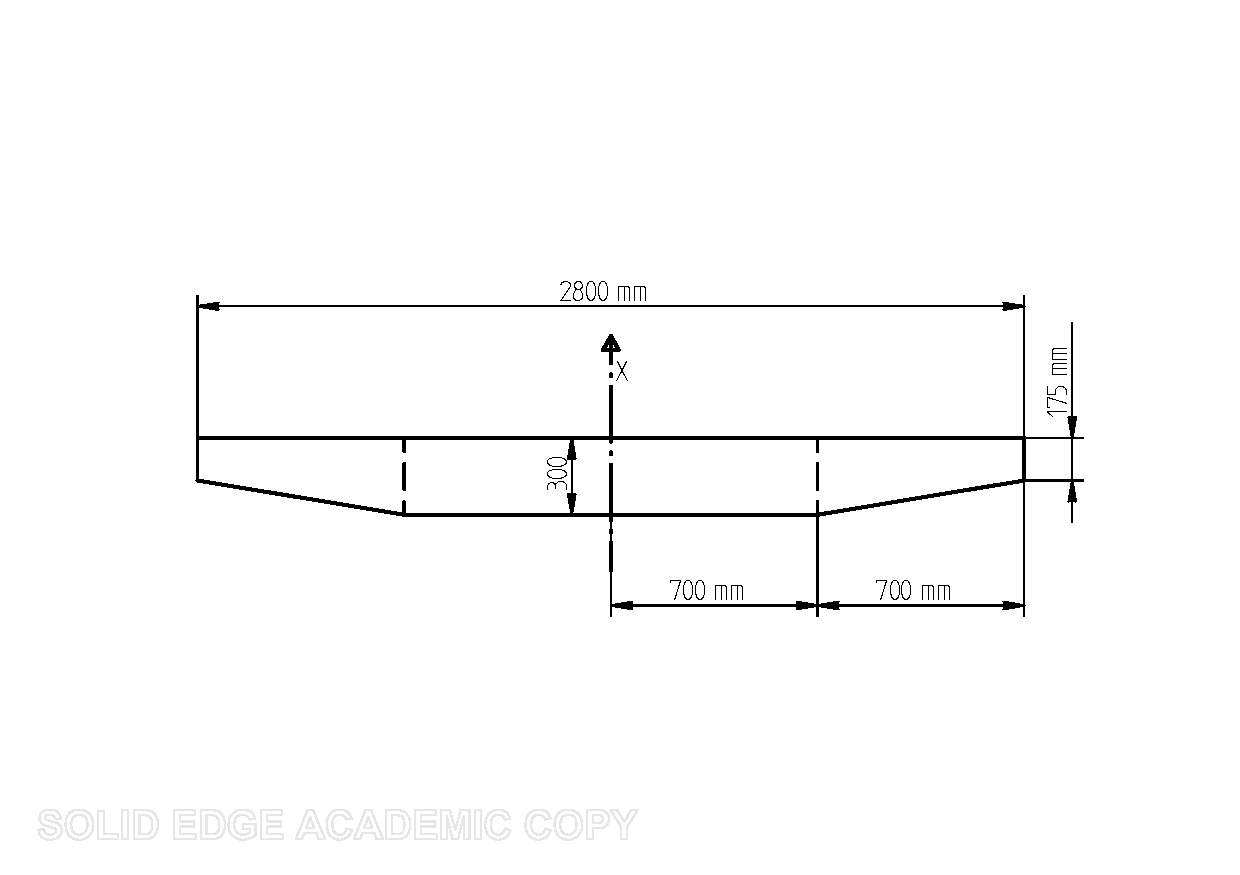
\includegraphics[width=0.9\textwidth, trim={15mm 40mm 15mm 40mm},clip]{bilder/Fotos/Grundriss_Flaeche.pdf}
\caption{Aufriss mit Eckdaten der Fläche} 
\label{fig:Flächenaufriss}
\end{figure}

Die Tragfläche setzt sich aus einem zentralen rechteckigen Segment und jeweils daran angeschlossenen Außensegmenten 
in Trapezform zusammen.
Hierbei werden Eigenschaften von bisher eingesetzten Flügeln übernommen.
Eine weitergehende Diskussion über die Wahl dieser aerodynamischen Parameter soll in dieser Arbeit nicht stattfinden. 
%\colorbox{red}{Es wird von der Strukturauslegung ausgegangen.}
Die Wahl von geradlinig aufgebauten Tragflächensegmenten ermöglicht hier Vorteile bei der Fertigung.\\
Im Bild \ref{fig:Flächenaufriss} ist ein Aufriss mit den Grundabmessungen dargestellt,welche für die aerodynamische Berechnung und den mechanischen Aufbau verwendet werden.

\begin{table}[h]
\centering
\begin{tabular}{|l|l|l|l|}
\hline
Parameter  & Bezeichnung &  Wert & Einheit \\ \hline
Spannweite  & $V_{reise}$ & 2800 & $mm$\\ \hline
Projizierte Fläche & $A_{ref}$  & 0,752 & $m^2$\\ \hline
Wurzeltiefe & $CH_{Wurzel}$ & 300 & $mm$ \\ \hline
Spitzenverwindung & $\alpha_{Spitze}$ & -\,2 & $^\circ$\\ \hline
Mittlere Flügeltiefe & $l_{\mu}$ & 275 & $mm$ \\ \hline
\end{tabular}
\caption{Dimensionen des Tragflügels}
\label{tab:Dimensionen des Tragflügels}
\end{table}

\clearpage


\section{Bestimmung der Lasten}
Mit einem Gewicht von 5,0 kg gehört das Fluggerät gemäß CS 23 der Kategorie \glqq Normal\grqq{} an.
Alle Auslegungsrechnungen beziehen sich auf diese Eingliederung.


\subsection{Lasten im stationären Flug}
Im Folgenden zeigt die Abbildung \ref{fig:Stationärer Reiseflug in XFLR} den aeroynamischen Entwurf im stationär ausgelegten Reiseflug.

\begin{figure}[H]
\centering
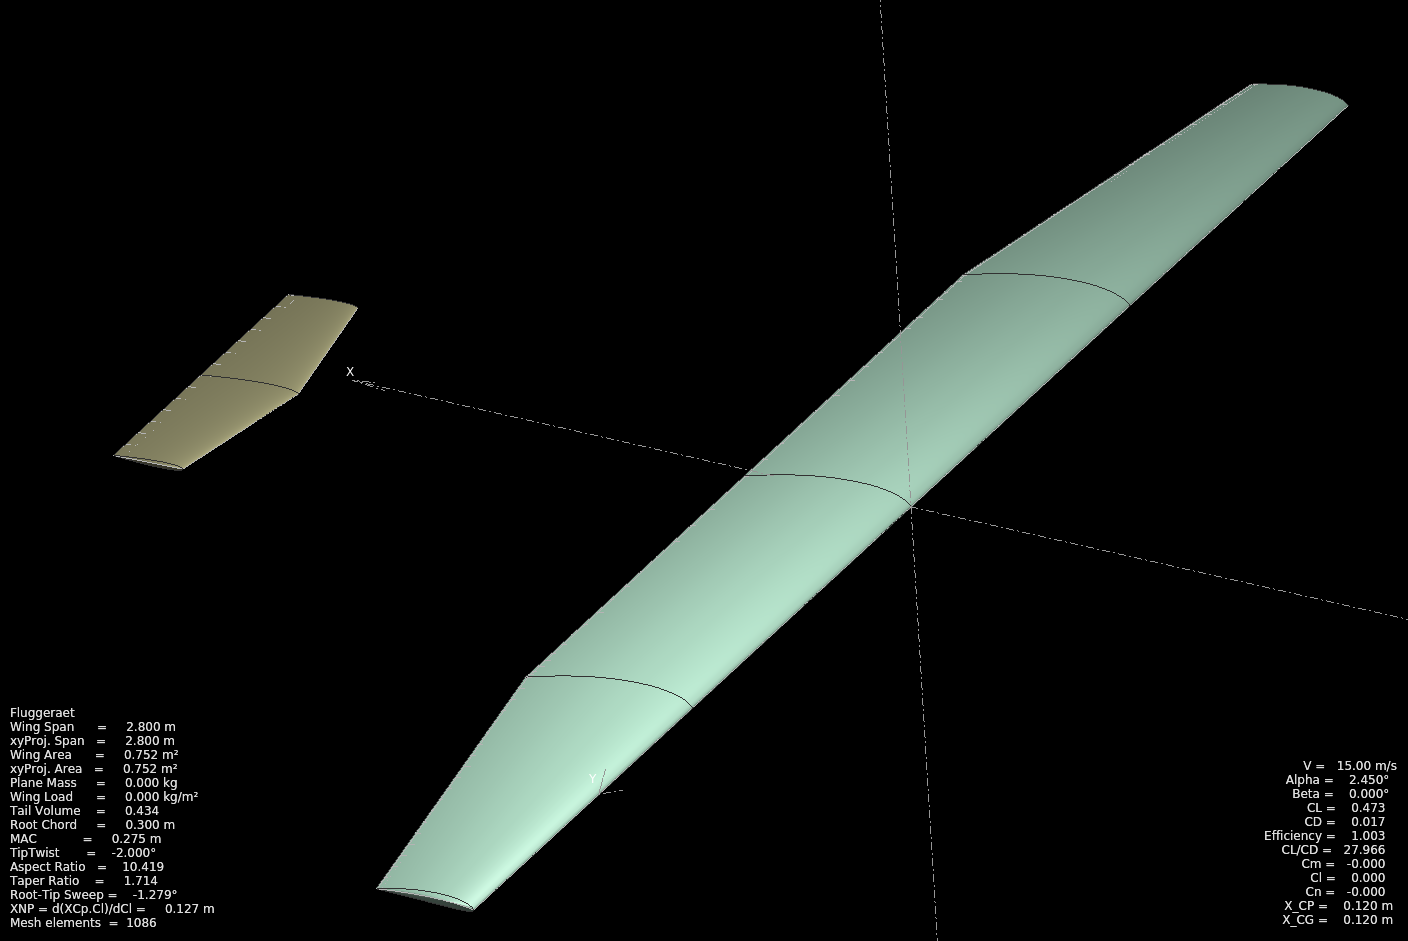
\includegraphics[width=0.9\textwidth]{bilder/Fotos/Aeroentwurf_Fluegelkonstruktion.png}
\caption{Stationärer Reiseflug bei 15 $m/s$ - entnommen den Berechnung in XFLR} 
\label{fig:Stationärer Reiseflug in XFLR}
\end{figure}

In diesem Fall ergibt die Ermittlung der aerodynamischen Beiwerte folgende Situation:

\begin{table}[h]
\centering
\begin{tabular}{|l|l|l|l|}
\hline
Parameter  & Bezeichnung &  Wert & Einheit \\ \hline
Fluggeschwindigkeit  & $V_{reise}$ & 15,00 & $m/s$\\ \hline
Abfluggewicht & $m_{reise}$  & 5,0 & $kg$\\ \hline
Anstellwinkel & $\alpha$ & 2,45 & $^\circ$ \\ \hline
Auftriebsbeiwert & $C_{L}$ & 0,473 & -\\ \hline
Widerstandsbeiwert & $C_{D}$ & 0,016  & -  \\ \hline
\end{tabular}
\caption{Errechnete Werte im stationären Reiseflug}
\label{tab:Errechnete Werte im Stationären Reiseflug}
\end{table}

In diesem Zustand ist der Flügel frei von Nickmomenten und das Höhenleitwerk erzeugt keine aerodynamischen Auftriebskräfte.

\clearpage

\subsection{Resultierende Kräfte und Momente}
\label{Resultierende Kräfte und Momenten Stationär}

In der stationären Flugsituation entstehen die folgenden maximalen Kräfte und Momente.

Biegemoment auf der 25\% Tiefenlinie der Tragfläche um die Einspannung in $Y = 0$
\begin{equation}
M_{b-X\,max} = 13,92 Nm    
\end{equation}

Drehmoment  um die 25\% Tiefenlinie an der Einspannung $Y = 0$
\begin{equation}
M_{t-Y\,max} \approx 0 Nm
\end{equation}
Für diesen Auslegungszustand ist der Schwerpunkt des Systems so gewähl, dass es im Arbeitspunkt nahezu momentenfrei fliegt. Das Höhenleitwerk kommt lediglich bei Abweichungen aus diesem Zustand zum Wirken.

\subsection{Kritische Lasten}

Gemäß CS 23.337 werden die positiven und negativen maximalen Manöverlastvielfachen berechnet.

Abflugmasse (take off weight) des Flugzeugs:
\begin{equation}
\label{eq:K1}
W_{0} = \SI{5}{\kilogram} = \SI{11,0231}{lb}
\end{equation}

Positive limit manoevering load factor:
\begin{equation}
\label{eq:K2}
n_{pos} = 2,1 + \frac{24000}{W_{0}+10000} = 4,4974 \qquad n_{pos gewählt}=4,5
\end{equation}

Negative limit manoevering load factor:
\begin{equation}
\label{eq:K3}
n_{neg} = (-0,4) \cdot n_{pos} = -1,7989 \qquad n_{neg_gewählt}=-1,8
\end{equation}

%/\begin{figure}[H]
%/\centering
%/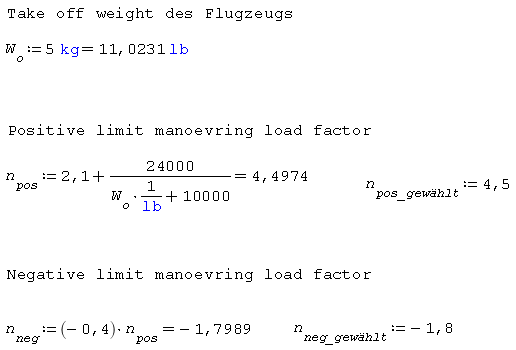
\includegraphics[width=0.9\textwidth]{bilder/Formeln/Kritische_Lastfaelle_Manoeverlasten.png}
%/\caption{Limit manoevring load factors nach CS23.337} 
%/\label{fig:Limit manoevring load factors nach CS23.337}
%/\end{figure}

%/Hochstart

%/Hier soll in konservativer Auslegung der Lasten für den gegebenfalls belastendensten Fall beim Hochstart mittels Gummiseil abgeschätzt werden. Hier übersteigt die Auftriebsbelastung für den Hochanstellwinkelbereich kurzeitig den Maximalauftrieb des Profils durch den Betrieb im instationären Bereich./%

%\\subsection{\colorbox{red}{Resultierende Kräfte und Momente}}
\label{Resultierende Kräfte und Momenten Kritisch}

\clearpage

\section{Betriebsgrenzen des Tragflügels}

Im Einsatz unterliegt das Tragwerk sowohl aerodynamischen als auch mechanischen Grenzen.
Diese werden Allgemein nach \cite{Sperl2011} berechnet.

Zunächst werden die kritischen Geschwindigkeiten für den Einsatz mit und ohne Klappen bestimmt:

\begin{equation}
\label{eq:K4}
c_{\text{L\ max\ Flap}} = 1.5 \qquad c_{\text{L\ max\ Clean}} = 1.3 
\end{equation}

\begin{equation}
\label{eq:K5}
V_{\text{S\,0}} = \sqrt{\cfrac{W_{0\ \text{MTOW}} \cdot \SI[per-mode = fraction]{9,81}{\meter\squared\per\second\squared}}{c_{\text{L\ max\ Flap}} \cdot \cfrac{\rho_{\text{Luft\ 0m}}}{2} \cdot S_{Wing}}}=\SI[per-mode = fraction]{8,42581}{\meter\per\second} \qquad V_{\text{S\,0\ gewählt}}=\SI[per-mode = fraction]{8,5}{\meter\per\second}
\end{equation}

\begin{equation}
\label{eq:K6}
V_{\text{stall\ gewählt}} = \sqrt{\cfrac{W_{0\ \text{MTOW}} \cdot \SI[per-mode = fraction]{9,81}{\meter\squared\per\second\squared}}{c_{\text{L\ max\ Clean}} \cdot \cfrac{\rho_{\text{Luft\ 0m}}}{2} \cdot S_{Wing}}}=\SI[per-mode = fraction]{9,05078}{\meter\per\second} \qquad V_{\text{stall\ gewählt}}=\SI[per-mode = fraction]{9,1}{\meter\per\second}
\end{equation}

%/\begin{figure}[H]
%/\centering
%/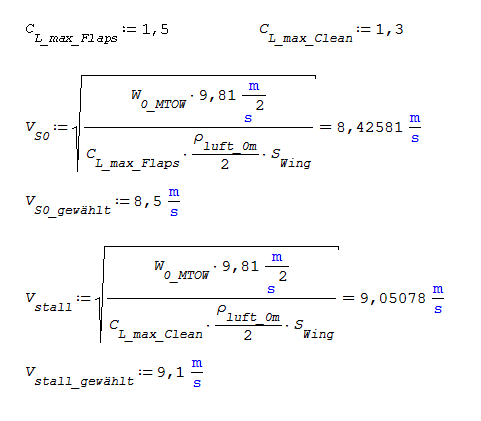
\includegraphics[width=0.9\textwidth]{bilder/Formeln/Mindestbetriebsgeschwindikeit.png}
%/\caption{Kritische Fluggeschwindikeiten} 
%/\label{fig:Kritische Fluggeschwindikeiten}
%/\end{figure}

Im selben Verfahren wird die Abrissgeschwindikeit (stall speed) für negative Werte des Auftriebs bestimmt:

\begin{equation}
\label{eq:K7}
c_{\text{L\ min\ Clean}} = 0.8 
\end{equation}
\begin{equation}
\label{eq:K8}
V_{\text{S\,neg}} = \sqrt{\cfrac{W_{0\ \text{MTOW}} \cdot \SI[per-mode = fraction]{9,81}{\meter\squared\per\second\squared}}{c_{\text{L\ min\ Clean}} \cdot \cfrac{\rho_{\text{Luft\ 0m}}}{2} \cdot S_{Wing}}}=\SI[per-mode = fraction]{11,53752}{\meter\per\second} \qquad V_{\text{S\,neg\ gewählt}}=\SI[per-mode = fraction]{11,6}{\meter\per\second}
\end{equation}

%/\begin{figure}[H]
%/\centering
%/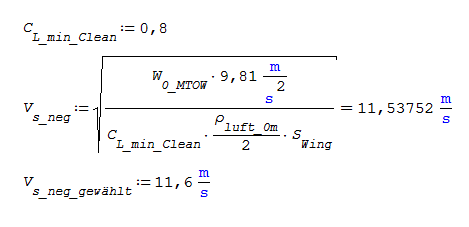
\includegraphics[width=0.9\textwidth]{bilder/Formeln/VS_neg.png}
%/\caption{Mindestgeschwindikeit für Invertierten Flug} 
%/\label{fig:Mindestgeschwindikeit für Invertierten Flug}
%/\end{figure}

Aus den Parametern ergibt sich im Weiteren die mindestens geforderte Höchstgeschwindigkeit beim Klappeneinsatz:

\begin{equation}
\label{eq:K8}
1.4 \cdot V_{\text{S\,0\ gewählt}}=\SI[per-mode = fraction]{11,9}{\meter\per\second} \quad
1.8 \cdot V_{\text{S\,0\ gewählt}}=\SI[per-mode = fraction]{16,38}{\meter\per\second} \quad
V_{\text{F\ gewählt}}=\SI[per-mode = fraction]{18}{\meter\per\second}
\end{equation}

%/\begin{figure}[H]
%/\centering
%/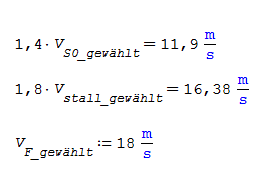
\includegraphics[width=0.9\textwidth]{bilder/Formeln/VF.png}
%/\caption{Klappenhöchstgeschwindigkeit} %/\label{fig:Klappenhöchstgeschwindigkeit}
%/\end{figure}

Des Weiteren ergeben sich die Manövergeschwindigkeiten $V_{A}$ und $V_{G}$ nach CS 23.335 zu:

\begin{equation}
\label{eq:K8}
V_{\text{A}}=V_{\text{S\,1\ gewählt}} \cdot \sqrt{n_{\text{pos}}}=\SI[per-mode = fraction]{19,304}{\meter\per\second} 
\end{equation}
\begin{equation}
\label{eq:K8}
V_{\text{G}}=V_{\text{S\,neg\ gewählt}} \cdot \sqrt{n_{\text{neg}}}=\SI[per-mode = fraction]{15,563}{\meter\per\second} 
\end{equation}

%/\begin{figure}[H]
%/\centering
%/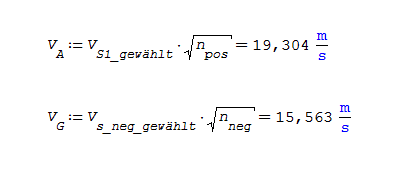
\includegraphics[width=0.9\textwidth]{bilder/Formeln/V_g.png}
%/\caption{Manövergeschwindigkeiten} 
%/\label{fig:Manövergeschwindigkeiten}
%/\end{figure}

\clearpage

Für den Dauerarbeitspunkt wird die Design Cruise Speed $V_{C}$ bestimmt:

\begin{equation}
\label{eq:K8}
W=\SI{11}{lb} \quad S=\SI{8,1}{ft^2}
\end{equation}
\begin{equation}
\label{eq:K8}
V_{\text{C\,min}}=33 \cdot \sqrt{\cfrac{W}{S}}=\SI{38,4563}{kn}=\SI[per-mode = fraction]{19,7804}{\meter\per\second}
\end{equation}
Berechnung von $V_{\text{C\,max}}$ entfällt mangels einer Leistungsauslegung
\begin{equation}
\label{eq:K8}
V_{\text{C\ gewählt}}=\SI[per-mode = fraction]{20}{\meter\per\second} 
\end{equation}

%/\begin{figure}[H]
%/\centering
%/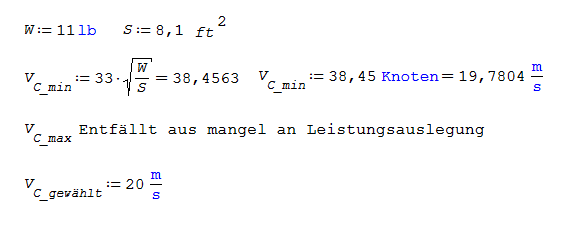
\includegraphics[width=0.9\textwidth]{bilder/Formeln/V_c.png}
%/\caption{Design Cruise Speed} 
%/\label{fig:Design Cruise Speed}
%/\end{figure}

Aus dieser lässt sich die maximal nicht zu überschreitende Geschwindigkeit $V_{D}$ ableiten:

\begin{equation}
\label{eq:K8}
V_{\text{D\,min\,1}}=1.25 \cdot V_{\text{C\,max}} \quad 
\end{equation}
Berechnung von $V_{\text{D\,min\,1}}$ entfällt mangels $V_{\text{C\,max}}$
\begin{equation}
\label{eq:K8}
V_{\text{D\,min\,2}}=1.35 \cdot V_{\text{C\ gewählt}}=\SI[per-mode = fraction]{27}{\meter\per\second} 
\end{equation}

%/\begin{figure}[H]
%/\centering
%/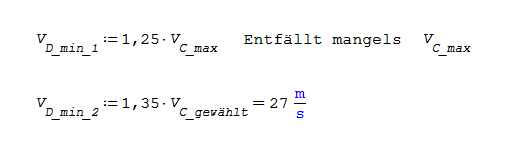
\includegraphics[width=0.9\textwidth]{bilder/Formeln/V_d.png}
%/\caption{Maximale Sturzgeschwindikeit} 
%/\label{fig:Maximale Sturzgeschwindikeit}
%/\end{figure}

\begin{landscape}
\begin{figure}[H]
\centering
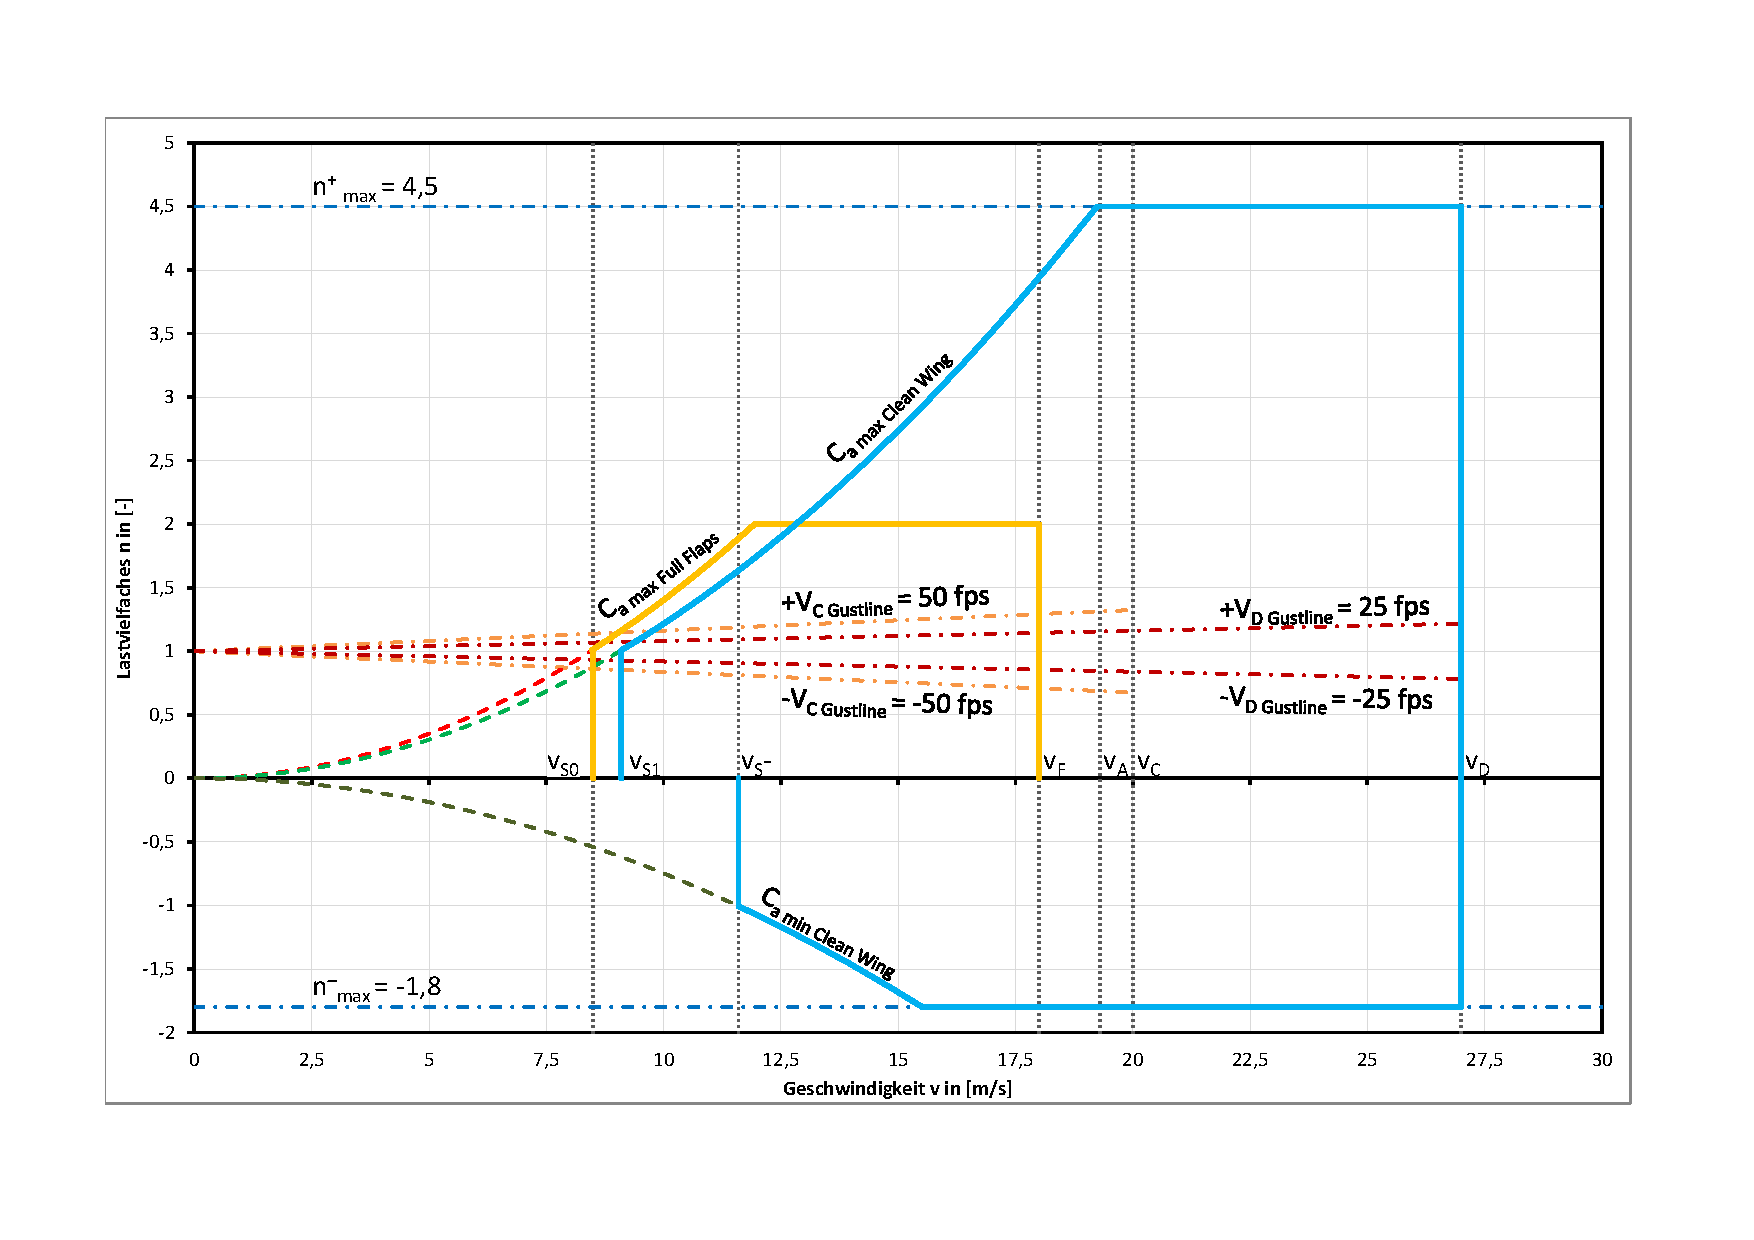
\includegraphics[height=0.945\textheight, trim={20mm 24mm 22mm 22mm},clip]{bilder/Formeln/VN-Diaggramm-rev-00.pdf}
\caption{Betriebsbereich im V\textsubscript{n}-Diagramm} 
\label{fig:Vn Diagramm des Flugsystems}
\end{figure}
\end{landscape}

%\cleardoublepage

\chapter{Material und Bauartbedingte Grenzen der Optimierung}\label{cha:Material- und Bauartbedingte Grenzen der Optimierung}

\section{Grenzen durch die Materialwahl}

\section{Grenzen durch die Verarbeitungsmethoden}

%\cleardoublepage

\chapter{Betrachtung verschiedener Bauweisen}\label{cha:Statistische Betrachtung bisheriger Bauformen}

In diesem Kapitel werden verschiedene Strukturbauweisen verglichen und ihre Tauglichkeit für den vorgesehen Einsatz bewertet.

\section{Vergleich verschiedener Strukturgewichte}

Um eine Auswahl der Bauweise nach Gewichtsgesichtspunkten zu treffen werden in der Tabelle \ref{tab:Flächengewichte Für Modelltragflügel} verschiedene realisierte Bauweisen einer Flügelstruktur von Faserverbund bis Folienbespannter Rippenbauweise aufgelistet. Dabei wird zur Vergleichbarkeit das Strukturgewicht je Projezierter Fläche errechnet.

Unberücksichtigt bleibt hier die jeweilig Maximal ertragbare Last jeder einzelnen Ausführung wodurch lediglich ein Vergleich der realisierbaren Bauarten erfolgen kann.
\begin{table}
\centering
\begin{adjustbox}{angle=90}
\begin{tabular}{|l|l|l|l|l|l|l|l|l|l|l|l|}
\hline
Name des Fluegels              & Hersteller         & Spannweite [mm] & Flügel MAC [mm] & Wurzeltiefe [mm] & Flaeche [m²] & Gewicht [g] & Gewicht [kg] & Strukturgewicht [kg/m²] & Bauweise \\ \hline
Ultraleicht Hangsegler         & Benjamin Bachmaier & 641             & 170              & 170              & 0,109         & 42,2        & 0,0422       & 0,387                    & Balsarippen Folienbespannt Kieferholm \\\hline
Ultraleicht Motorflieger       & Jens Schmelkus     & 1000            & 192              & 192              & 0,192         & 83,5        & 0,0835       & 0,435                    & Kiefer Sperrholzrippen auf CFK-Rohren Folienbespannt  \\\hline
Moravia Parkflyer              & Moravia            & 1190            & 200              & 200              & 0,238         & 195,7       & 0,1957       & 0,822                    & Balsarippen, Balsa Doppel T-Träger Folienbespannt         \\\hline
Kartonflügel Masterarbeit     & Ingrid             & 1450            & 272              & 295              & 0,394         & 380         & 0,3800       & 0,963                    & Mehrschicht Wellkarton Folienbespannt                            \\\hline
Kartonflügel Testsample       & Ingrid             & 200             & 245              & 245              & 0,049         & 47,8        & 0,0478       & 0,976                    & Mehrschicht Wellkarton Folienbespannt                          \\\hline
AUVSI RippensegmentTestversion & Jens Schmelkus     & 700             & 300              & 300              & 0,210         & 251,5       & 0,2515       & 1,198                    & Ceiba Rippen mit CFK Rohrholm Folienbespannt                     \\\hline
Easy Star                      & Multiplex          & 720             & 200              & 200              & 0,144         & 211,7       & 0,2117       & 1,470                    & Geschäumtes Polystyrol mit Glasfaserohrholm                     \\\hline
AUVSI 2016                     & Fa. Gewalt         & 1495            & 250              & 250              & 0,374         & 745         & 0,7450       & 1,993                    & Polystyrolkern mit Abachifunier Beplankt                         \\\hline
Ecuador 2015                   & Helmut Birzer      & 695             & 252              & 252              & 0,175         & 375,7       & 0,3757       & 2,145                    & Polystyrolkern mit Abachifunier Beplankt                         \\\hline
Chernobyl 2016                 & Team AUVSI         & 690             & 370              & 370              & 0,255         & 633,1       & 0,6331       & 2,480                    & Polystyrolkern mit Abachifunier Beplankt CFK Rohr                \\\hline
DS-Carbonfläche               & Steffen Bieg       & 1500            & 208              & 245              & 0,290         & 852         & 0,8520       & 2,938                    & Kohlefaser SchalenbauweiseIn Kohlefaserform Negativ \\  \hline               
\end{tabular}
\end{adjustbox}
\caption{Flächengewichte Für Modelltragflügel}
\label{tab:Flächengewichte Für Modelltragflügel}
\end{table}

\section{Qualitativer Vergleich der Formen}

Um die gestellte Flugaufgabe mit der notwendingen Strukturellen Sicherheit zu erfüllen soll die Bauweise eine einfache Skalierbarkeit ihrer Tragenden Elemente ermöglichen.
Die Dabei eingesetzten Geometrien eignen sich bezüglich ihrer Verhältnisse zwischen Widerstandsmoment gegen Biegung sowie Torsion und eingesetzten Querschnitten unterschiedlich gut.


\section{Nötiger Fertigungsaufwand}

Zur Herstellung der Verschiedenen Bauweise ist ein zum Teil erheblich unterschiedlicher Produktionsaufwand von nöten. Insbesondere die Herstellung von Vorrichtungen und Formen unterscheidet sich zwischen den Methoden. 

%\cleardoublepage

\chapter{Berechnung der Struktur}\label{cha:Berechnung der Struktur}

\section{Aufteilung der Lasten nach CS}

\subsection{Biegelasten}

\subsection{Querkräfte}

\subsection{Torsionsmomente}


%\cleardoublepage

\chapter{Konstruktion des Vergleichssegments}\label{cha:Konstruktion des Vergleichssegments}

%\cleardoublepage

%\chapter{Zeichnungssatz des Vergleichssegments}\label{cha:Zeichnungssatz des Vergleichssegments}

%\cleardoublepage

%\chapter{\colorbox{red}{Bewertung der Ergebnisse}}\label{cha:Bewertung der Ergebnisse}





%\cleardoublepage

\newpage
%\pagenumbering{Roman}
%\setcounter{page}{\value{roemisch}}

%Biblio-Management
\bibliography{literatur/bib}

%
% Abbildungsverzeichnis
%
\listoffigures

%
% Tabellenverzeichnis
%
\listoftables

\clearpage


% Appendix, falls vorhanden
\appendix

\chapter{Anhang}

\begin{table}[H]
\centering
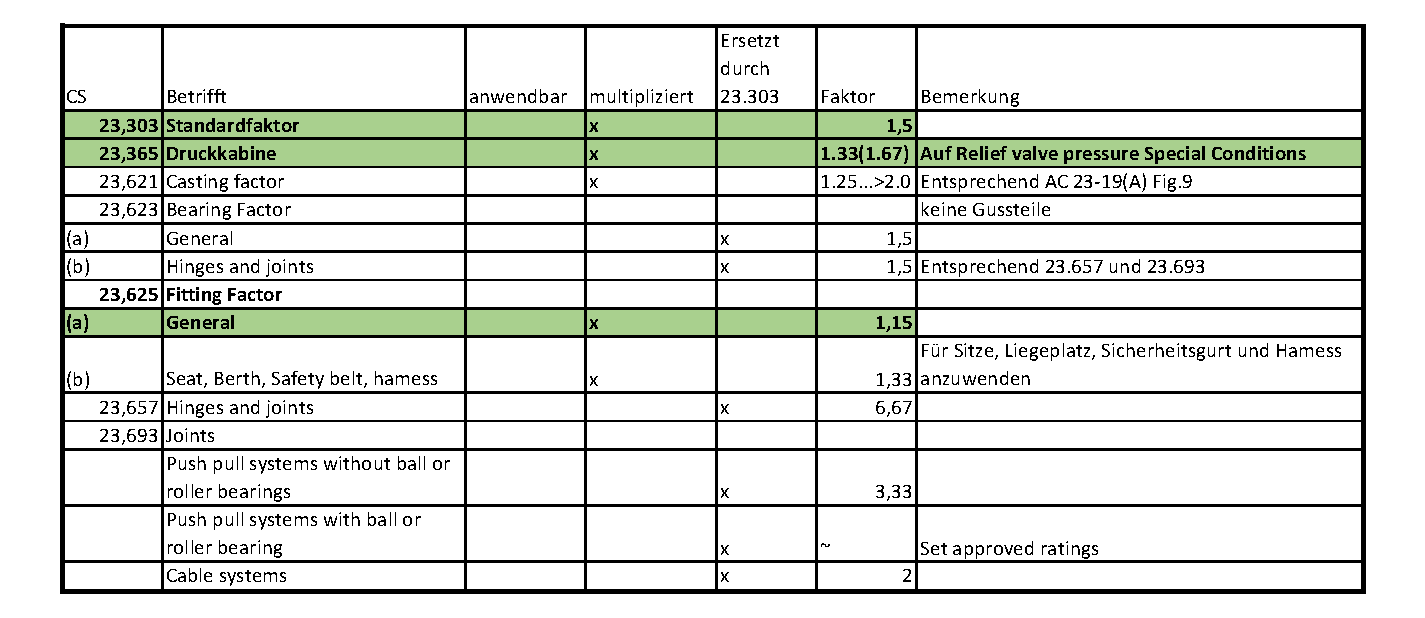
\includegraphics[width=0.9\textwidth]{bilder/Tabellen/Sicherheitsfaktoren.pdf}
\caption{Formblatt F021 - Nachweis der geforderten Sicherheit am Schnitt} 
\label{tab:Sicherheiten}
\end{table}

\clearpage

\begin{table}[H]
\centering
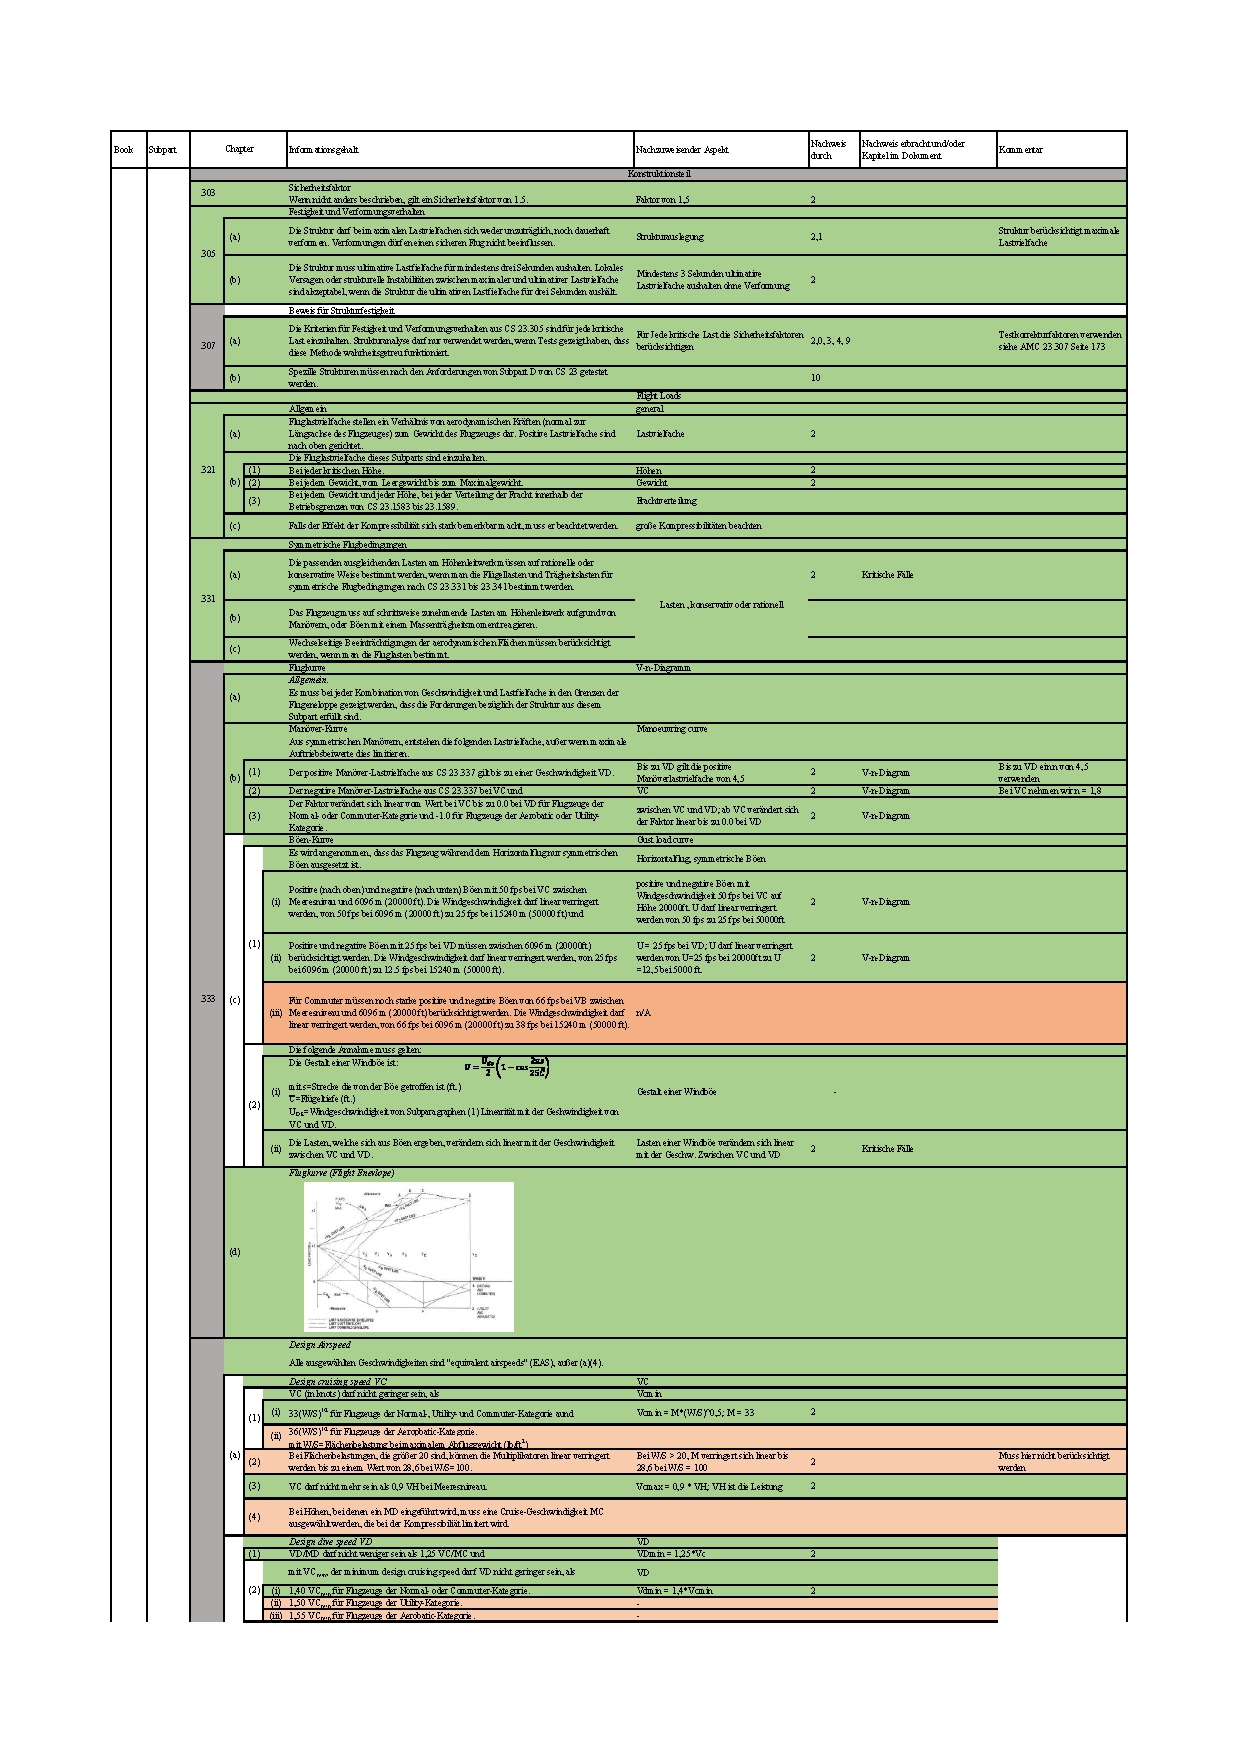
\includegraphics[width=0.9\textwidth]{bilder/Tabellen/MPP_Konstruktion_1.pdf}
\end{table}

\begin{table}[H]
\centering
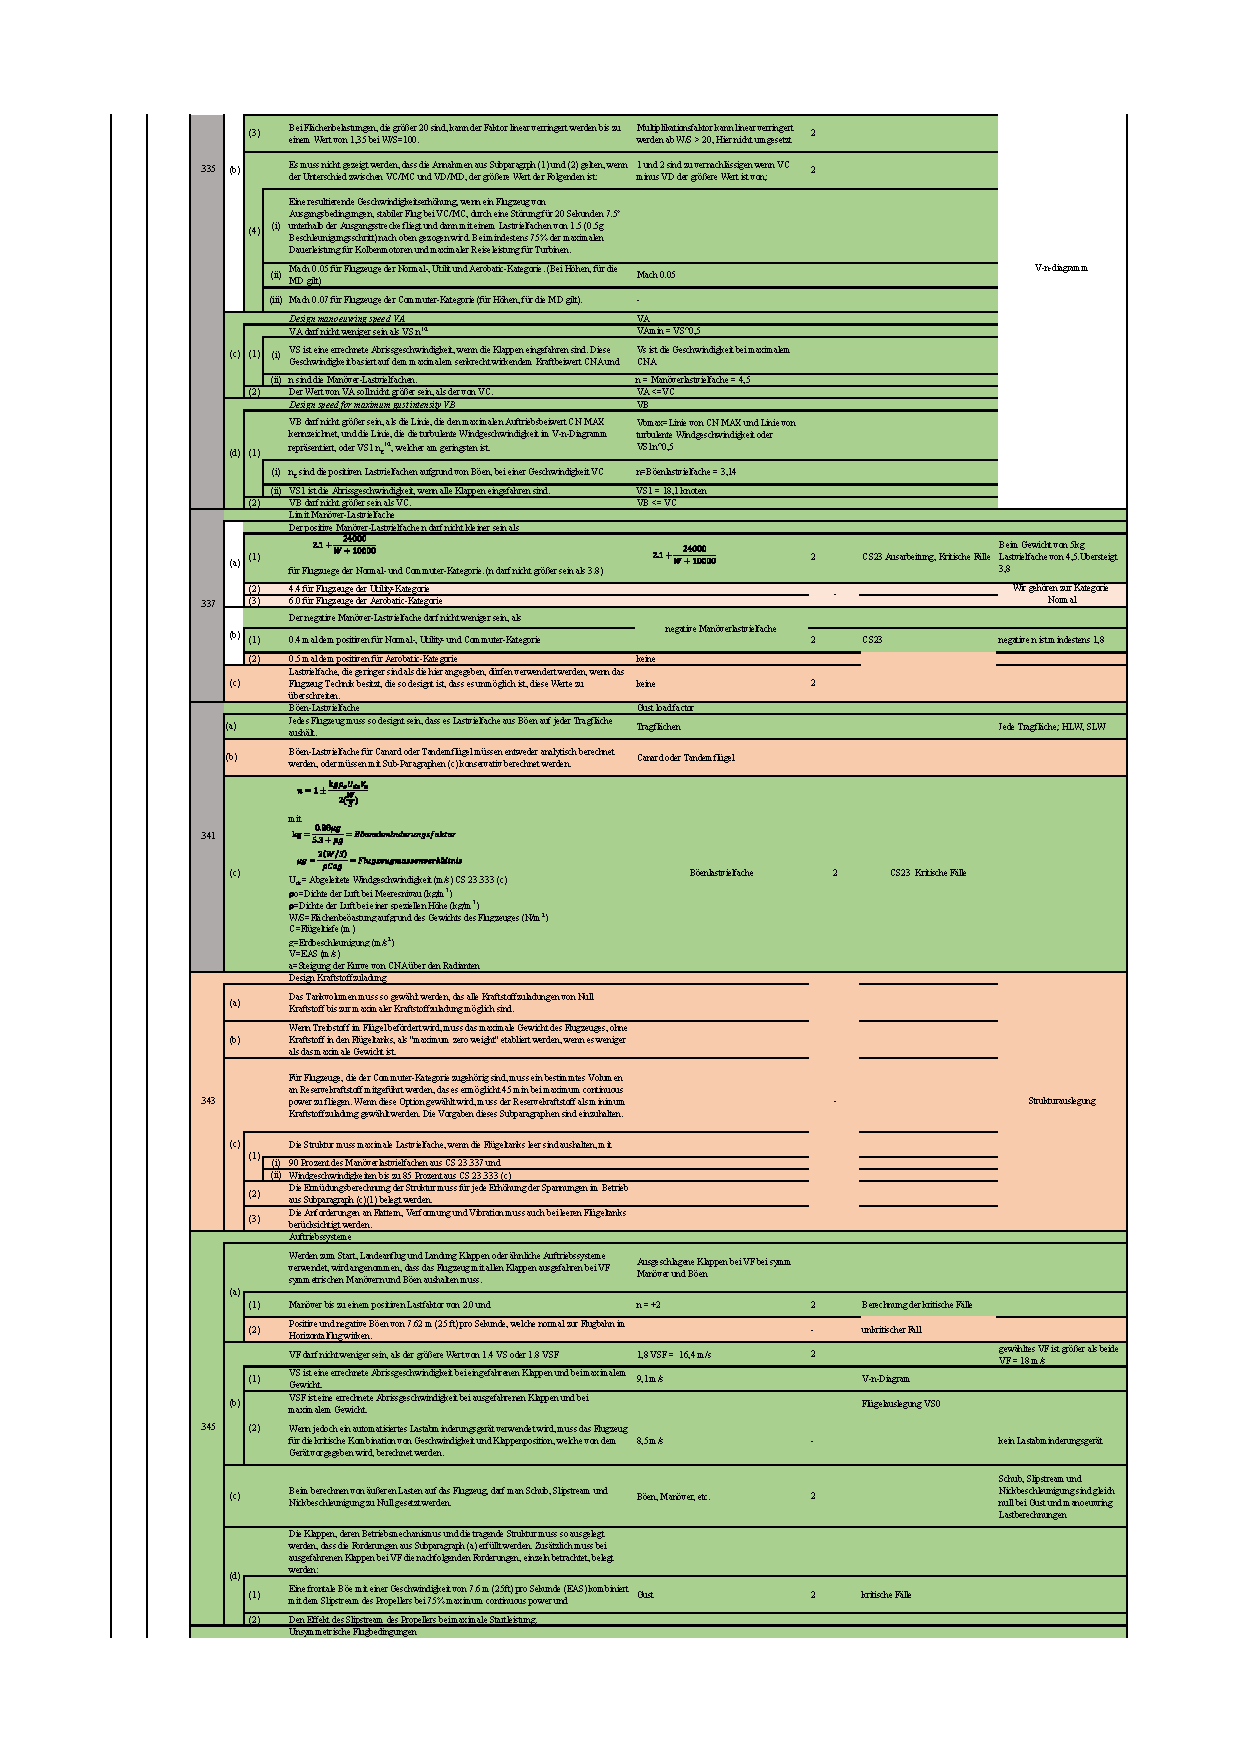
\includegraphics[width=0.9\textwidth]{bilder/Tabellen/MPP_Konstruktion_2.pdf}
\end{table}

\begin{table}[H]
\centering
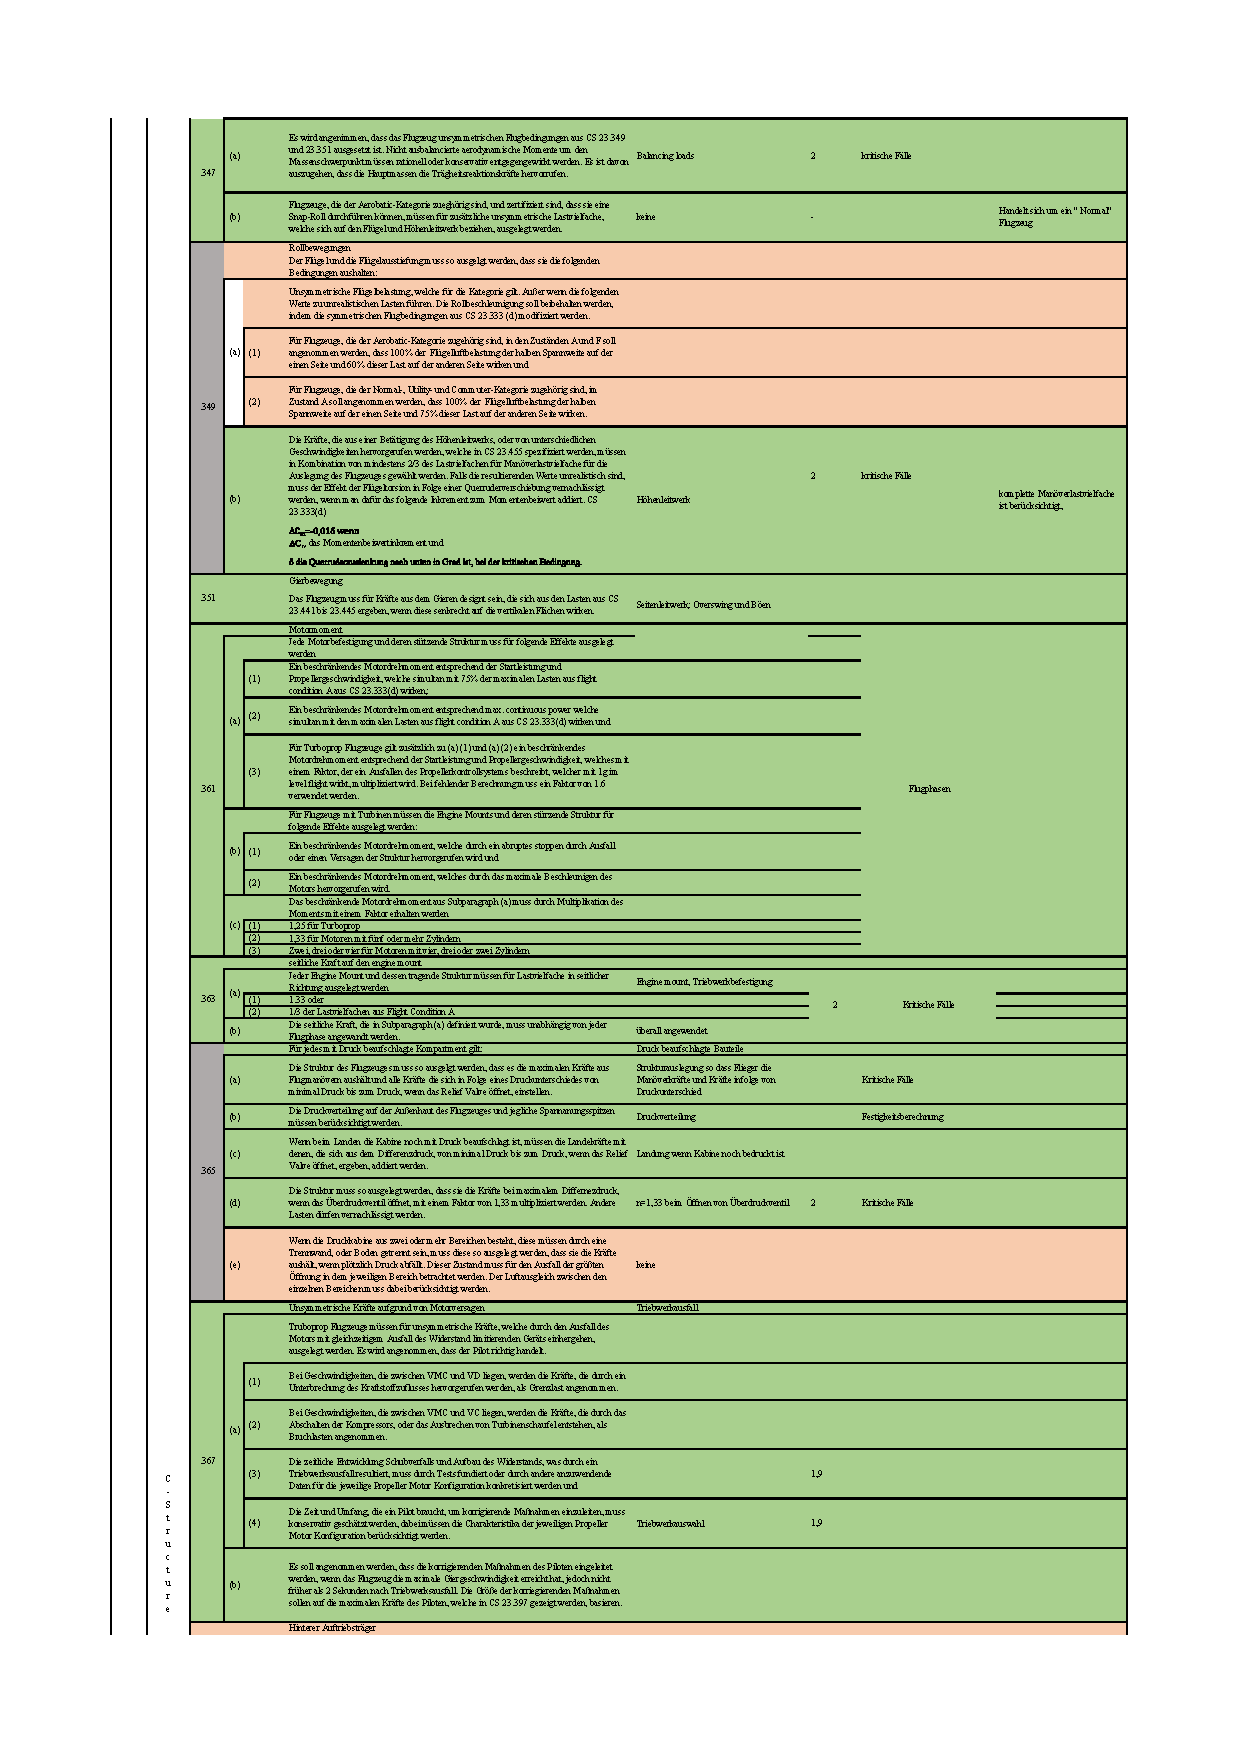
\includegraphics[width=0.9\textwidth]{bilder/Tabellen/MPP_Konstruktion_3.pdf}
\end{table}

\begin{table}[H]
\centering
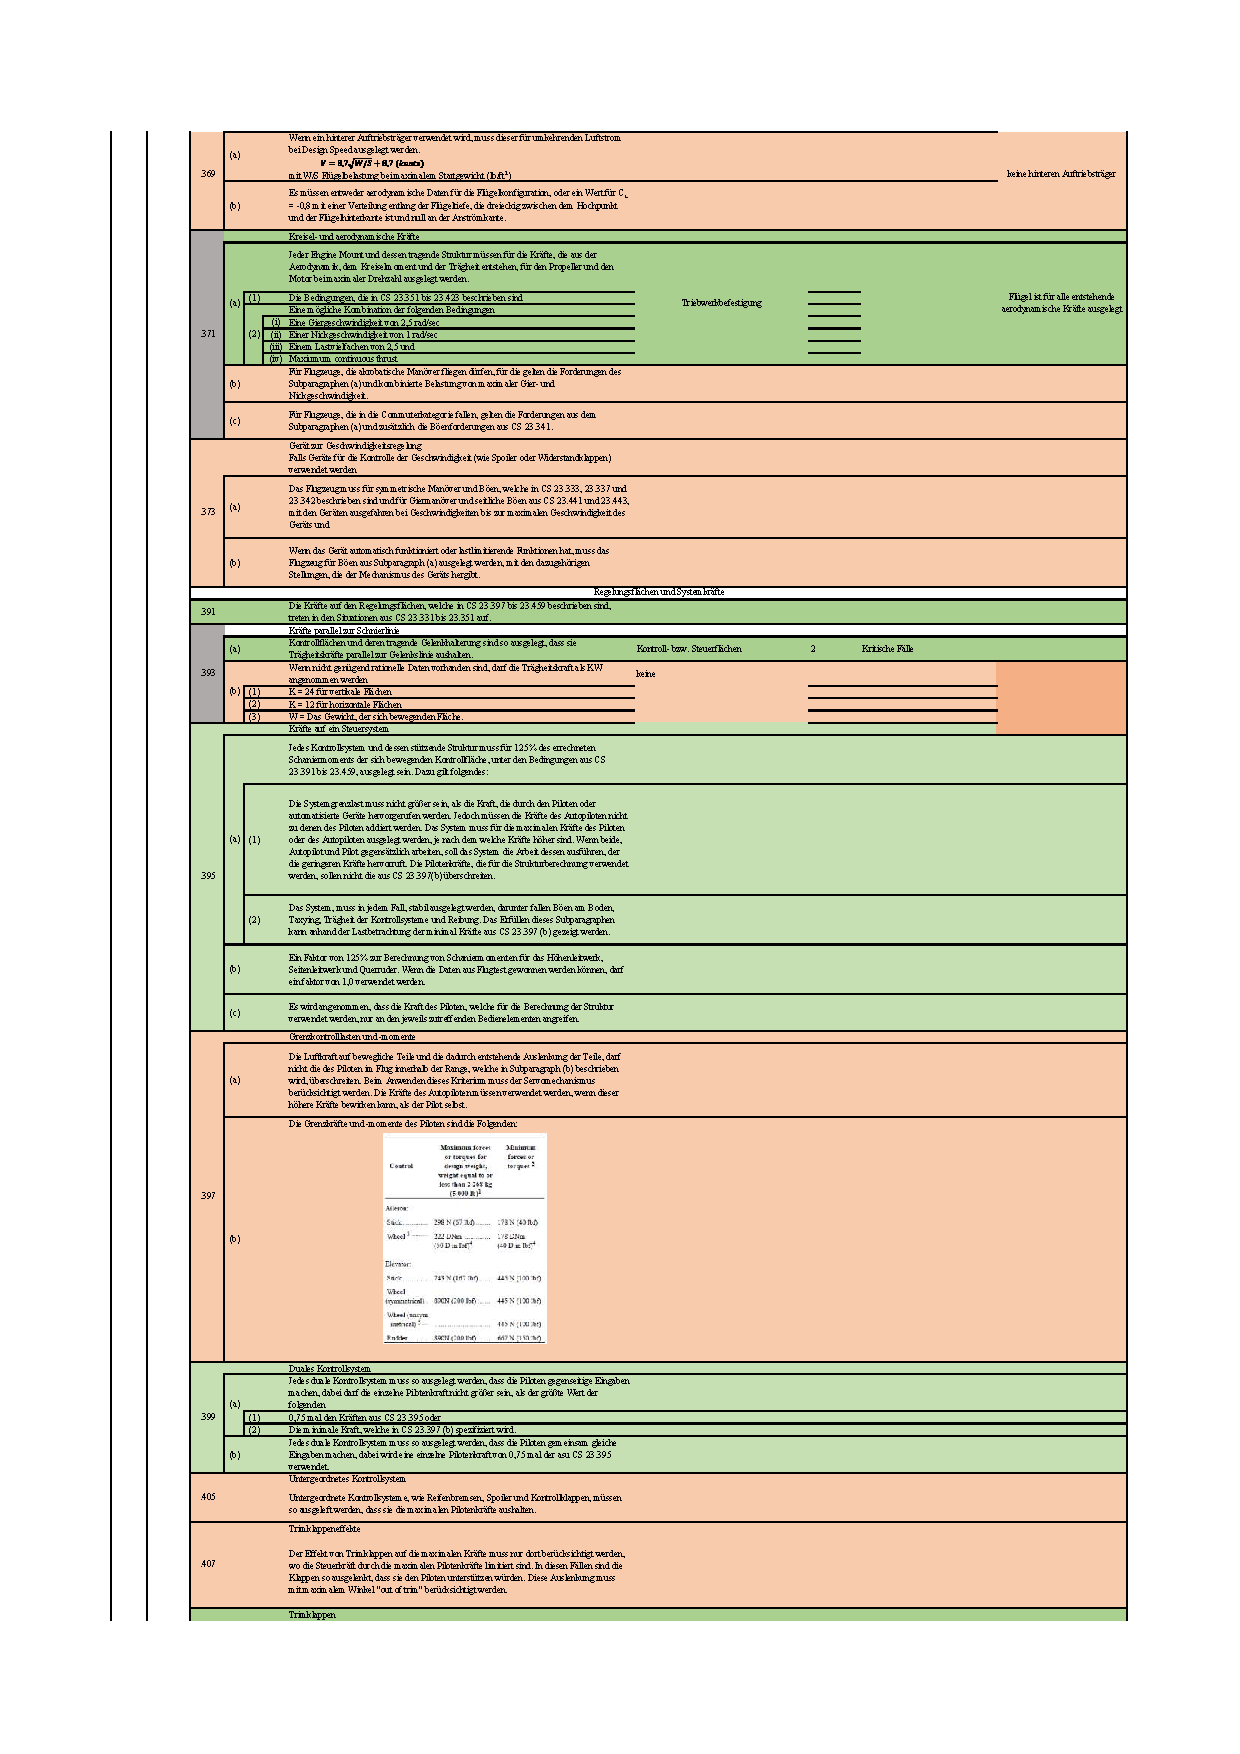
\includegraphics[width=0.9\textwidth]{bilder/Tabellen/MPP_Konstruktion_4.pdf}
\end{table}

\begin{table}[H]
\centering
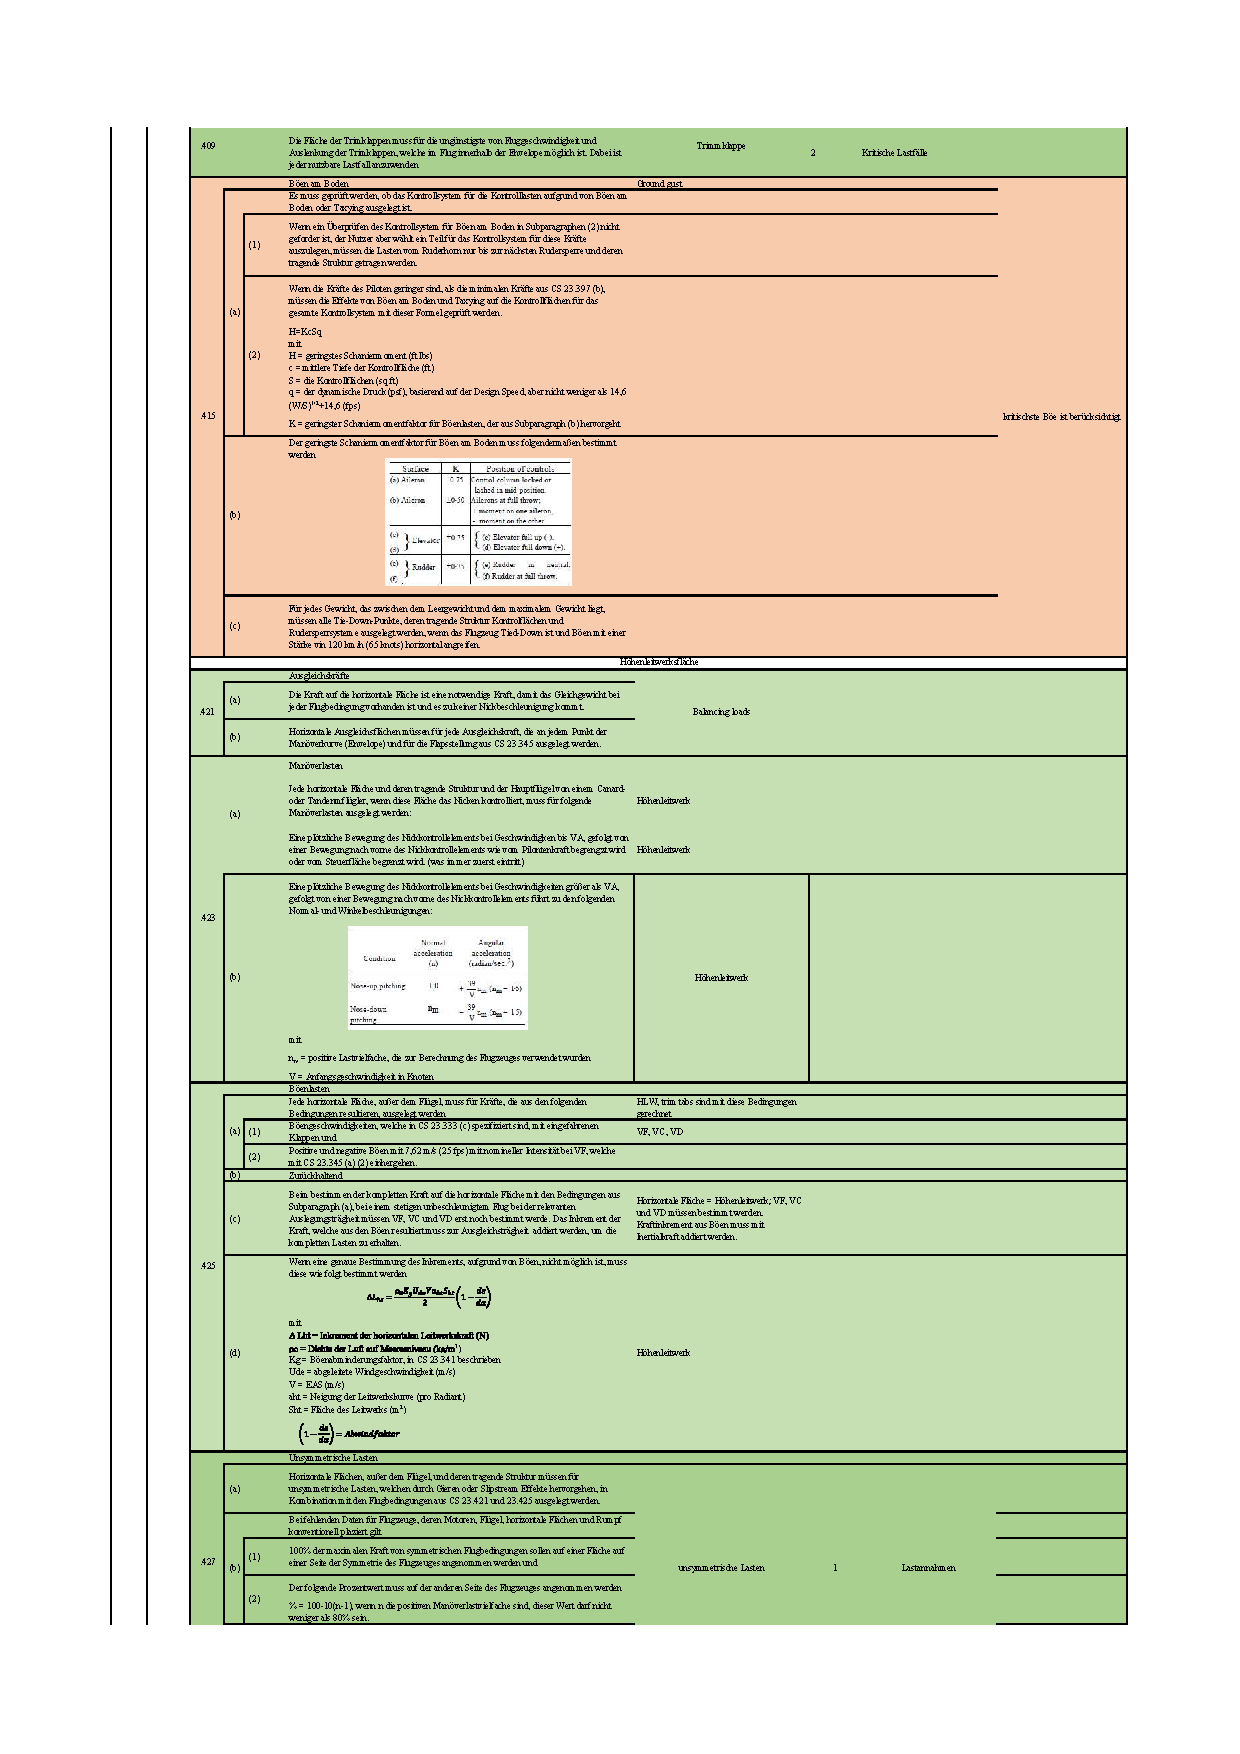
\includegraphics[width=0.9\textwidth]{bilder/Tabellen/MPP_Konstruktion_5.pdf}
\end{table}

\begin{table}[H]
\centering
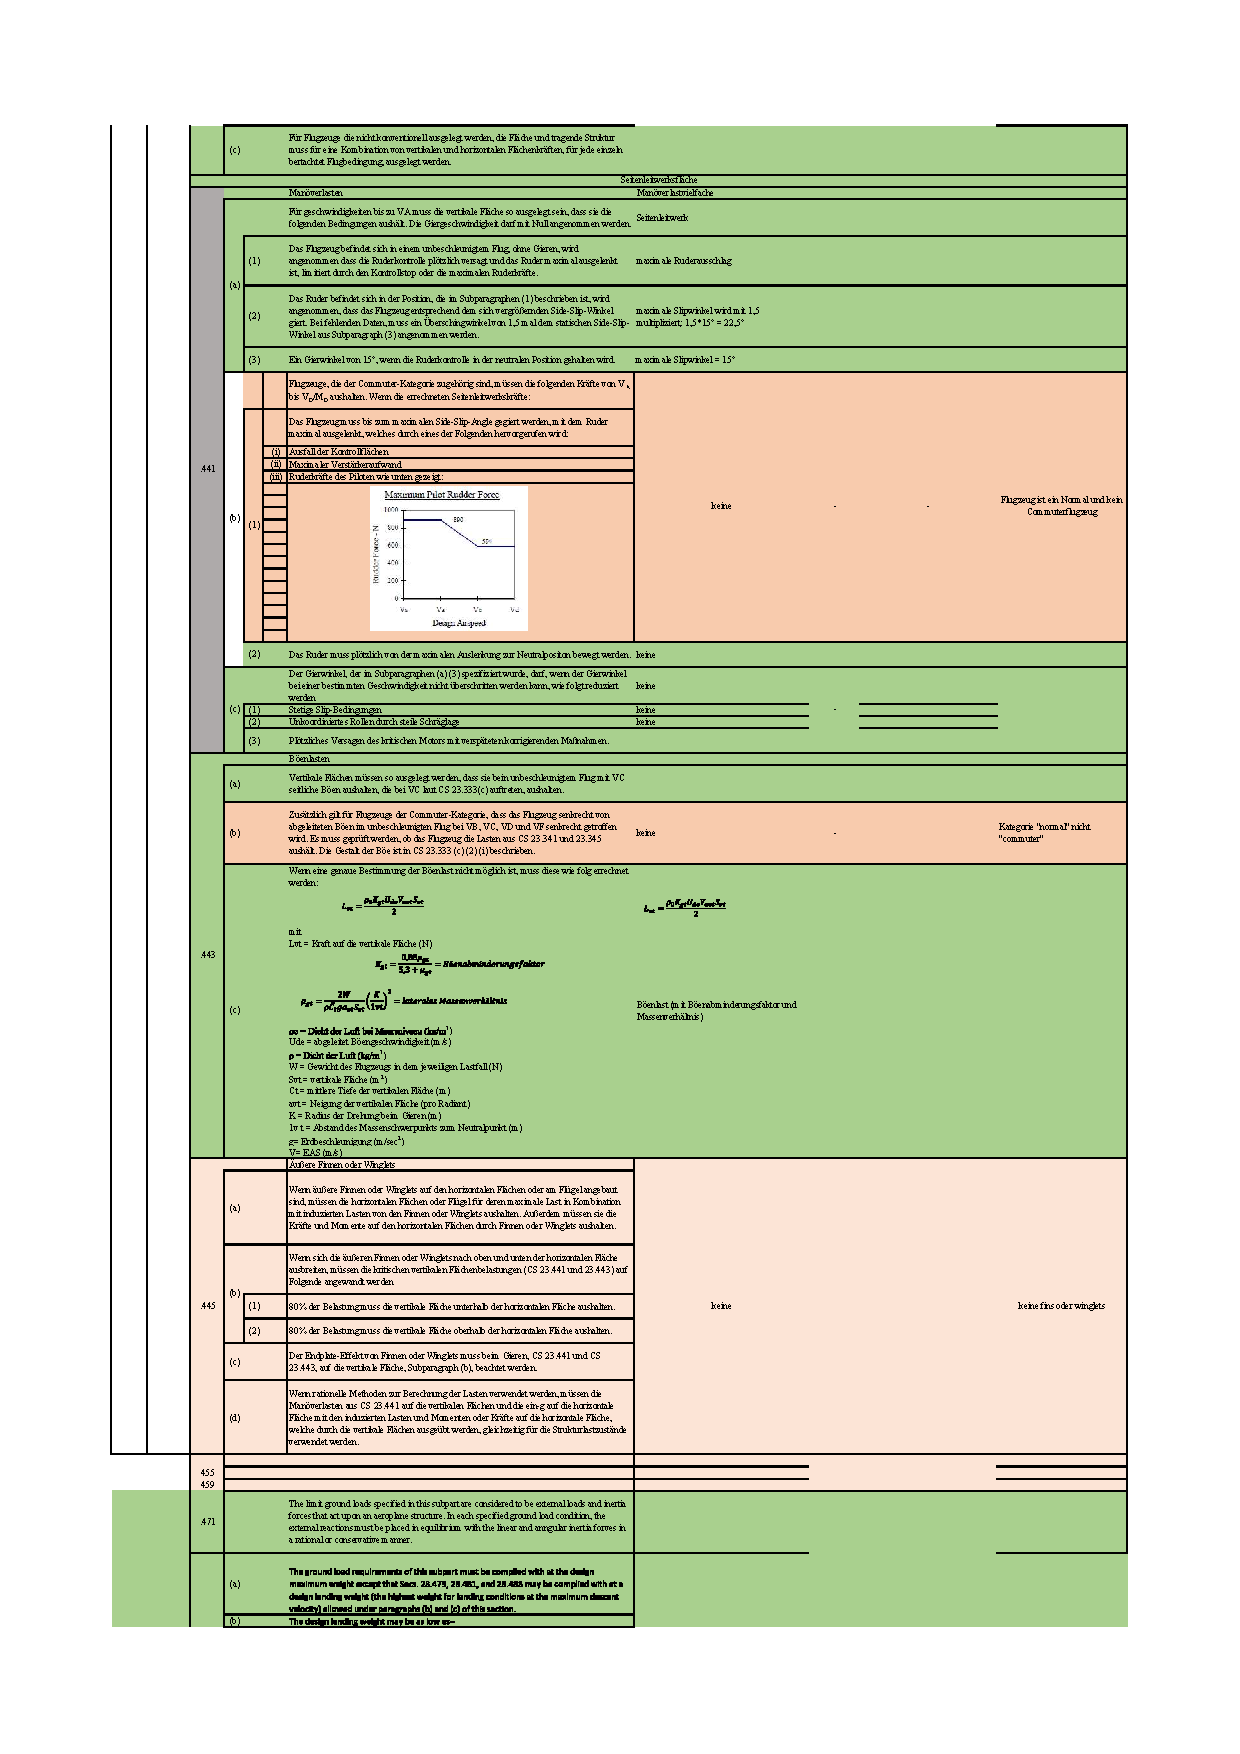
\includegraphics[width=0.9\textwidth]{bilder/Tabellen/MPP_Konstruktion_6.pdf}
\end{table}

\begin{table}[H]
\centering
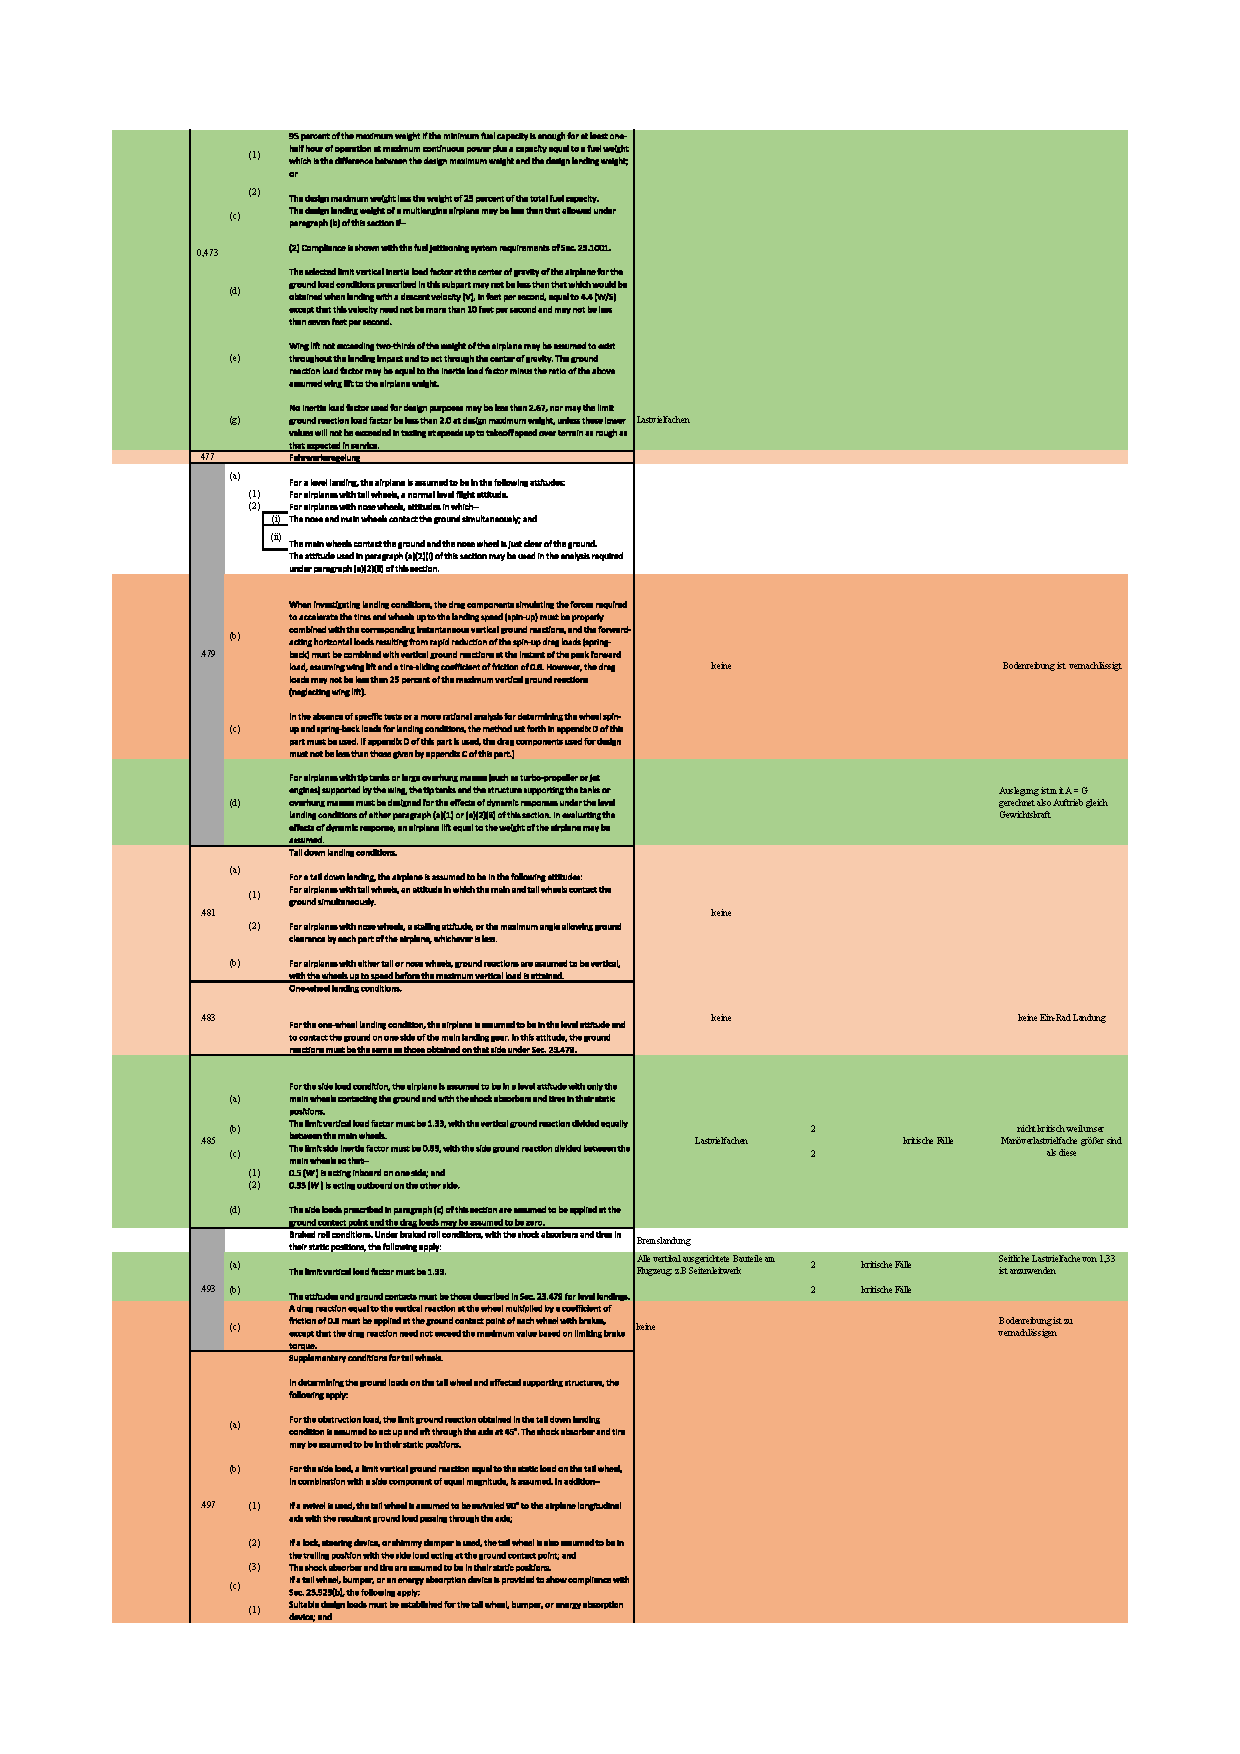
\includegraphics[width=0.9\textwidth]{bilder/Tabellen/MPP_Konstruktion_7.pdf}
\end{table}

\begin{table}[H]
\centering
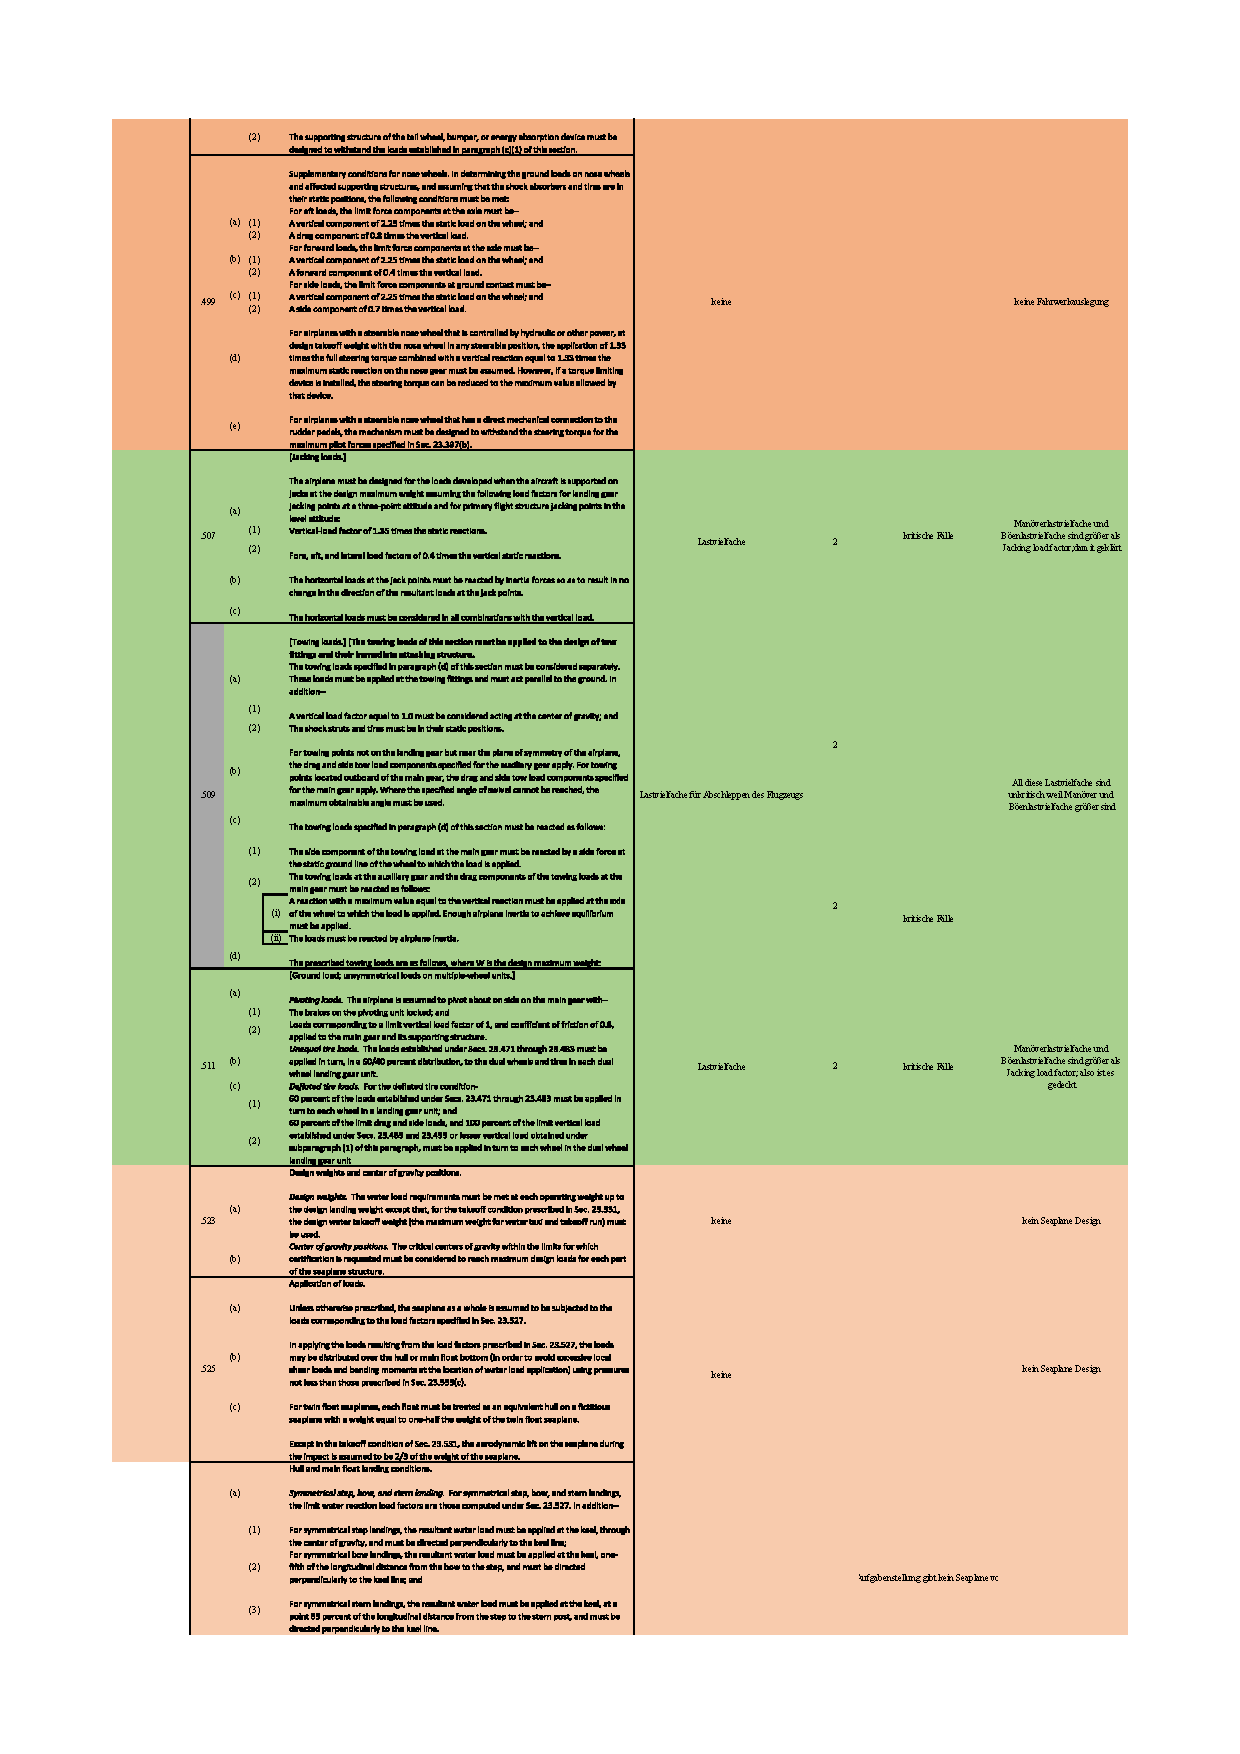
\includegraphics[width=0.9\textwidth]{bilder/Tabellen/MPP_Konstruktion_8.pdf}
\end{table}

\begin{table}[H]
\centering
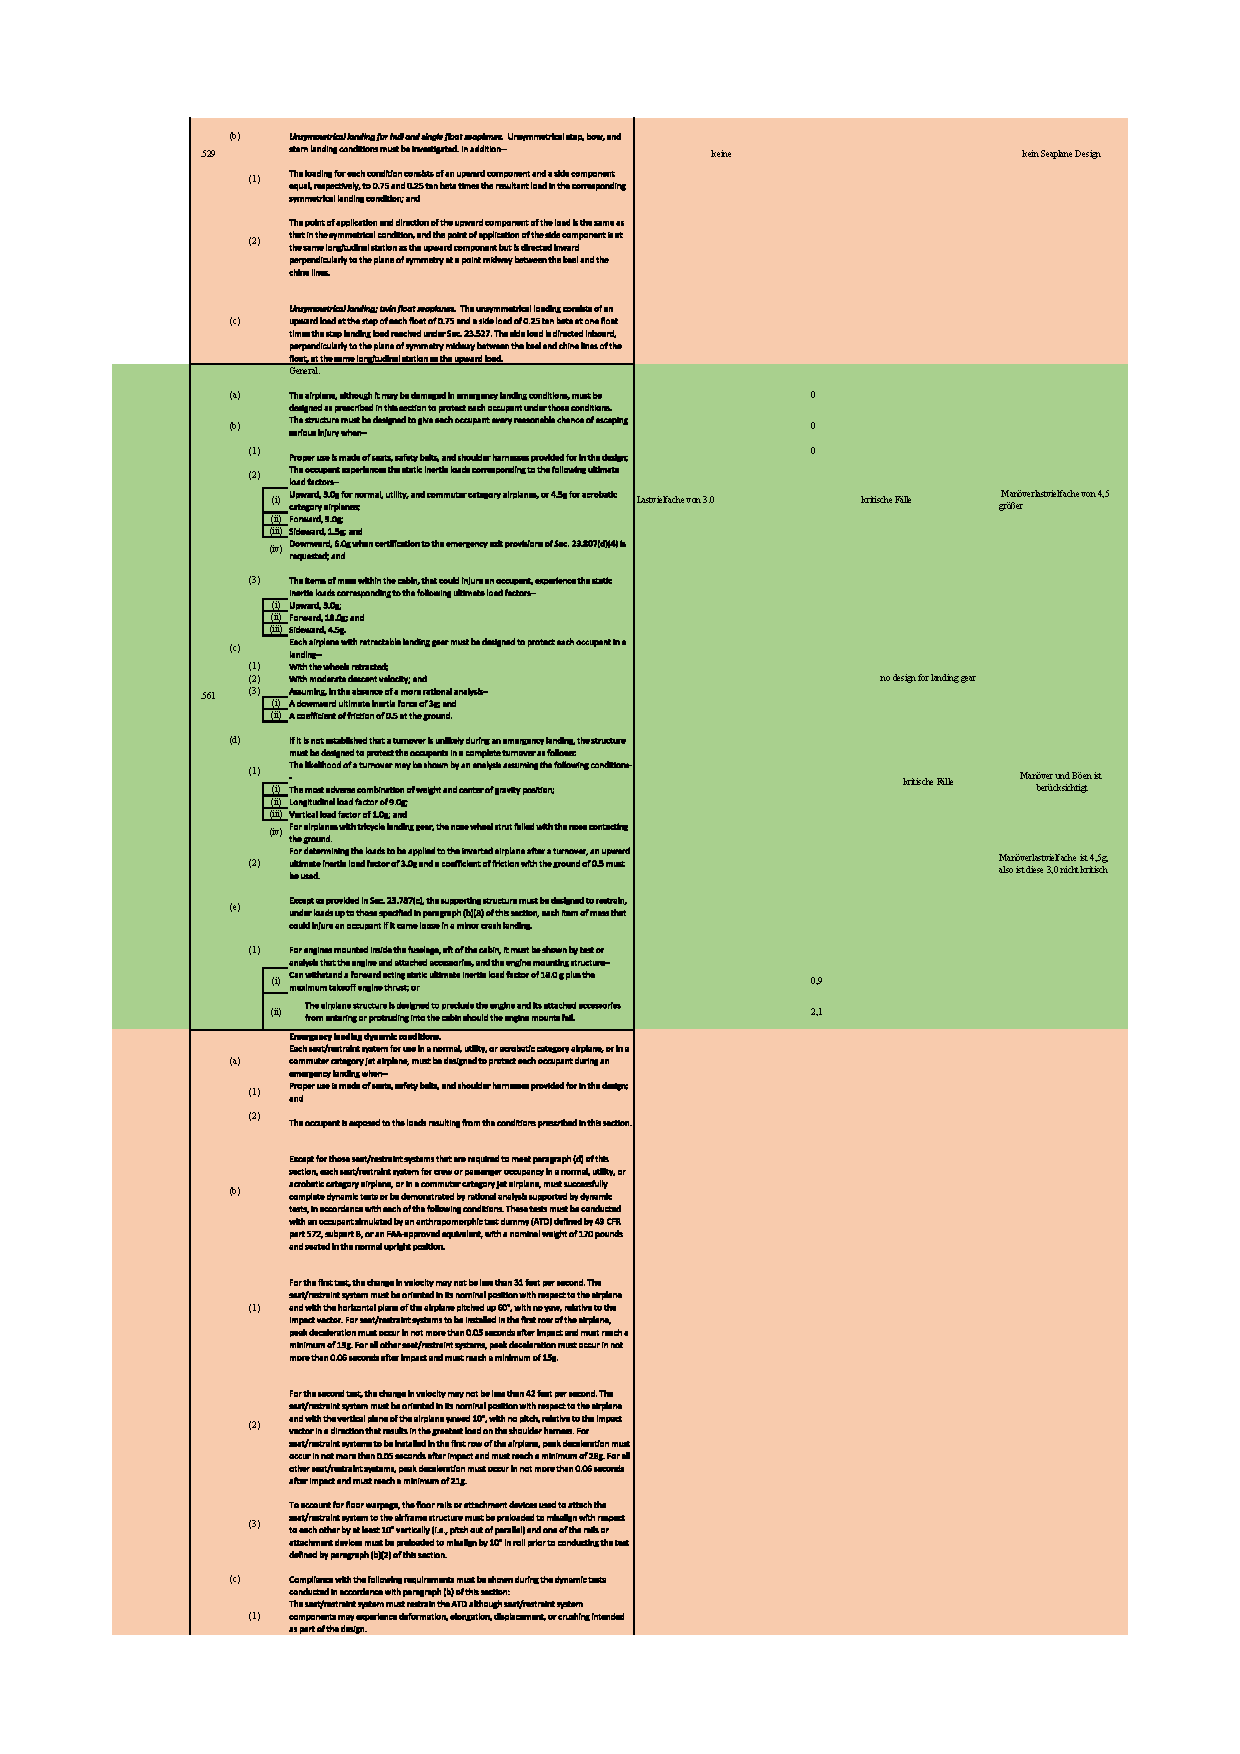
\includegraphics[width=0.9\textwidth]{bilder/Tabellen/MPP_Konstruktion_9.pdf}
\end{table}

\begin{table}[H]
\centering
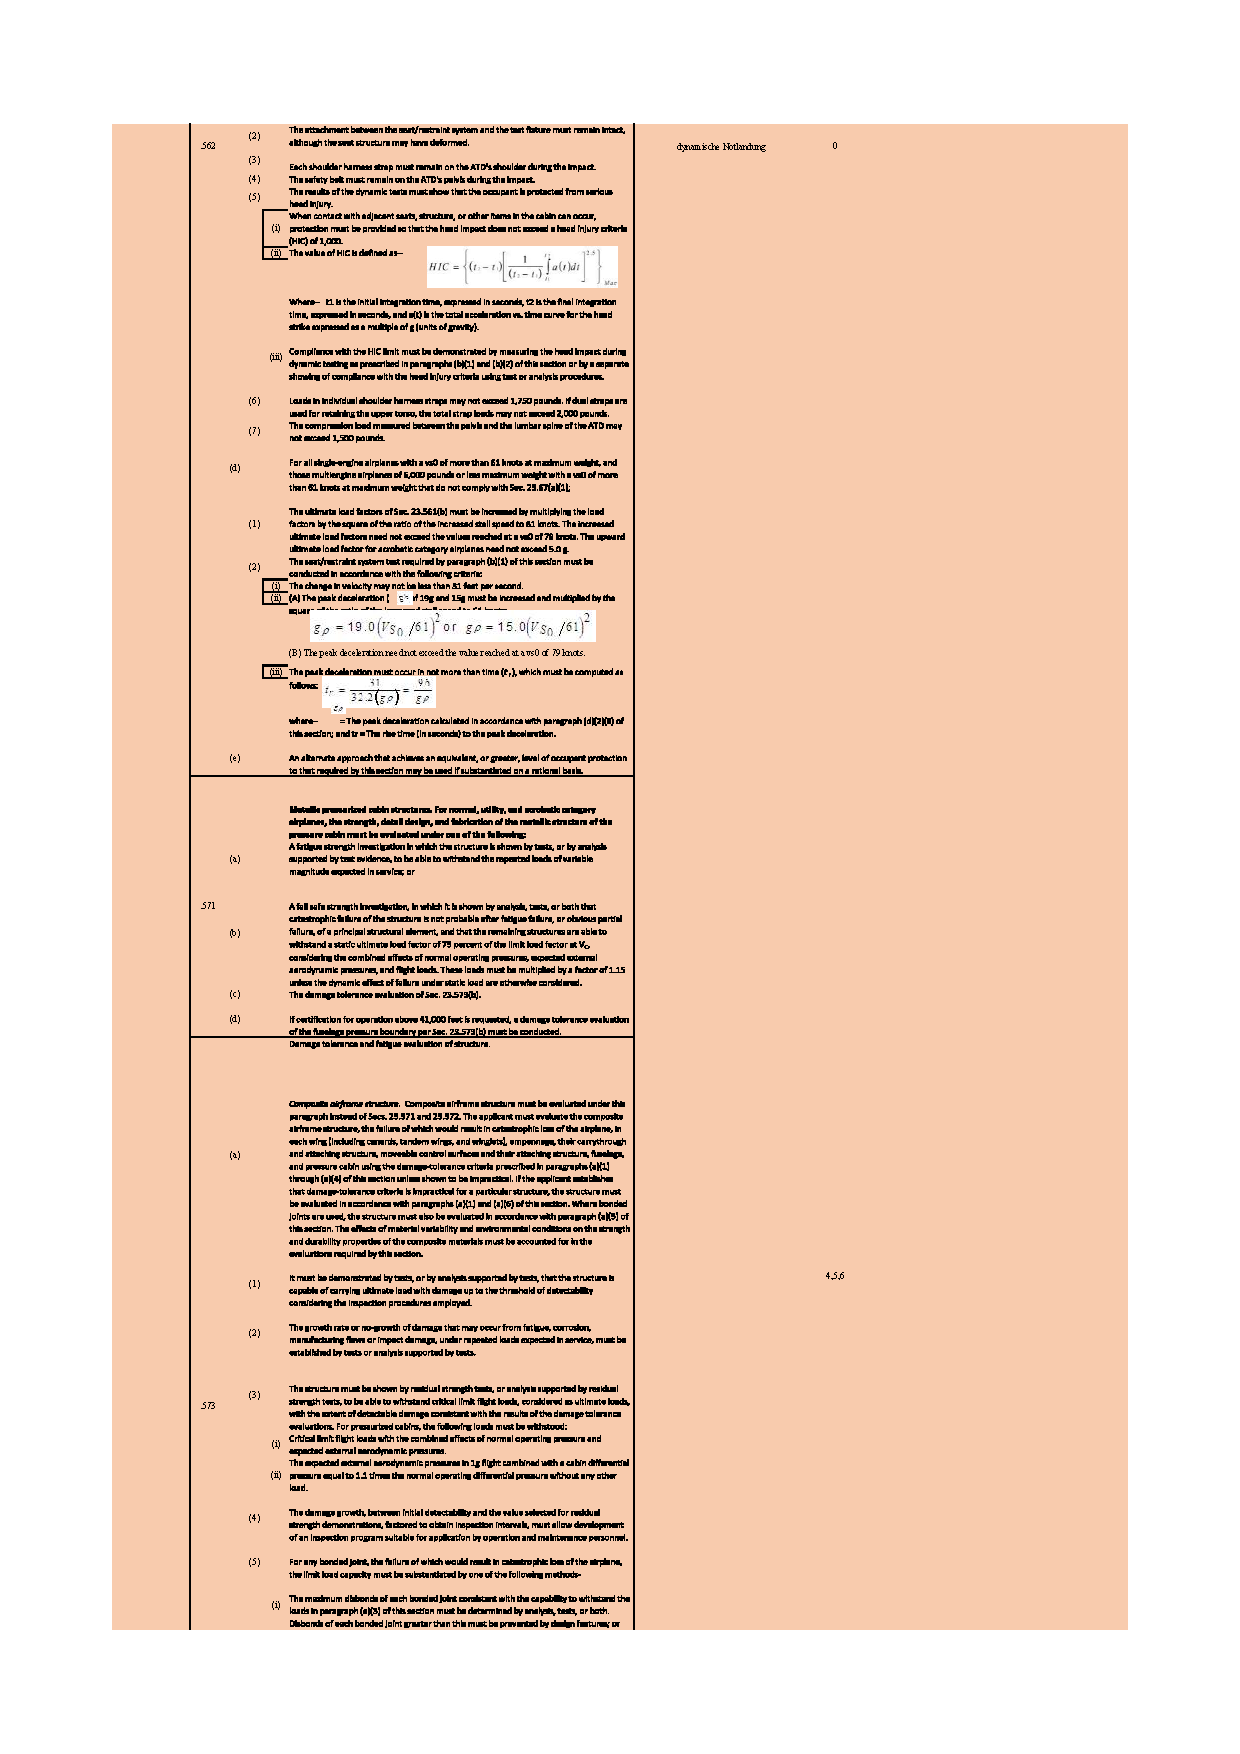
\includegraphics[width=0.9\textwidth]{bilder/Tabellen/MPP_Konstruktion_10.pdf}
\end{table}

\begin{table}[H]
\centering
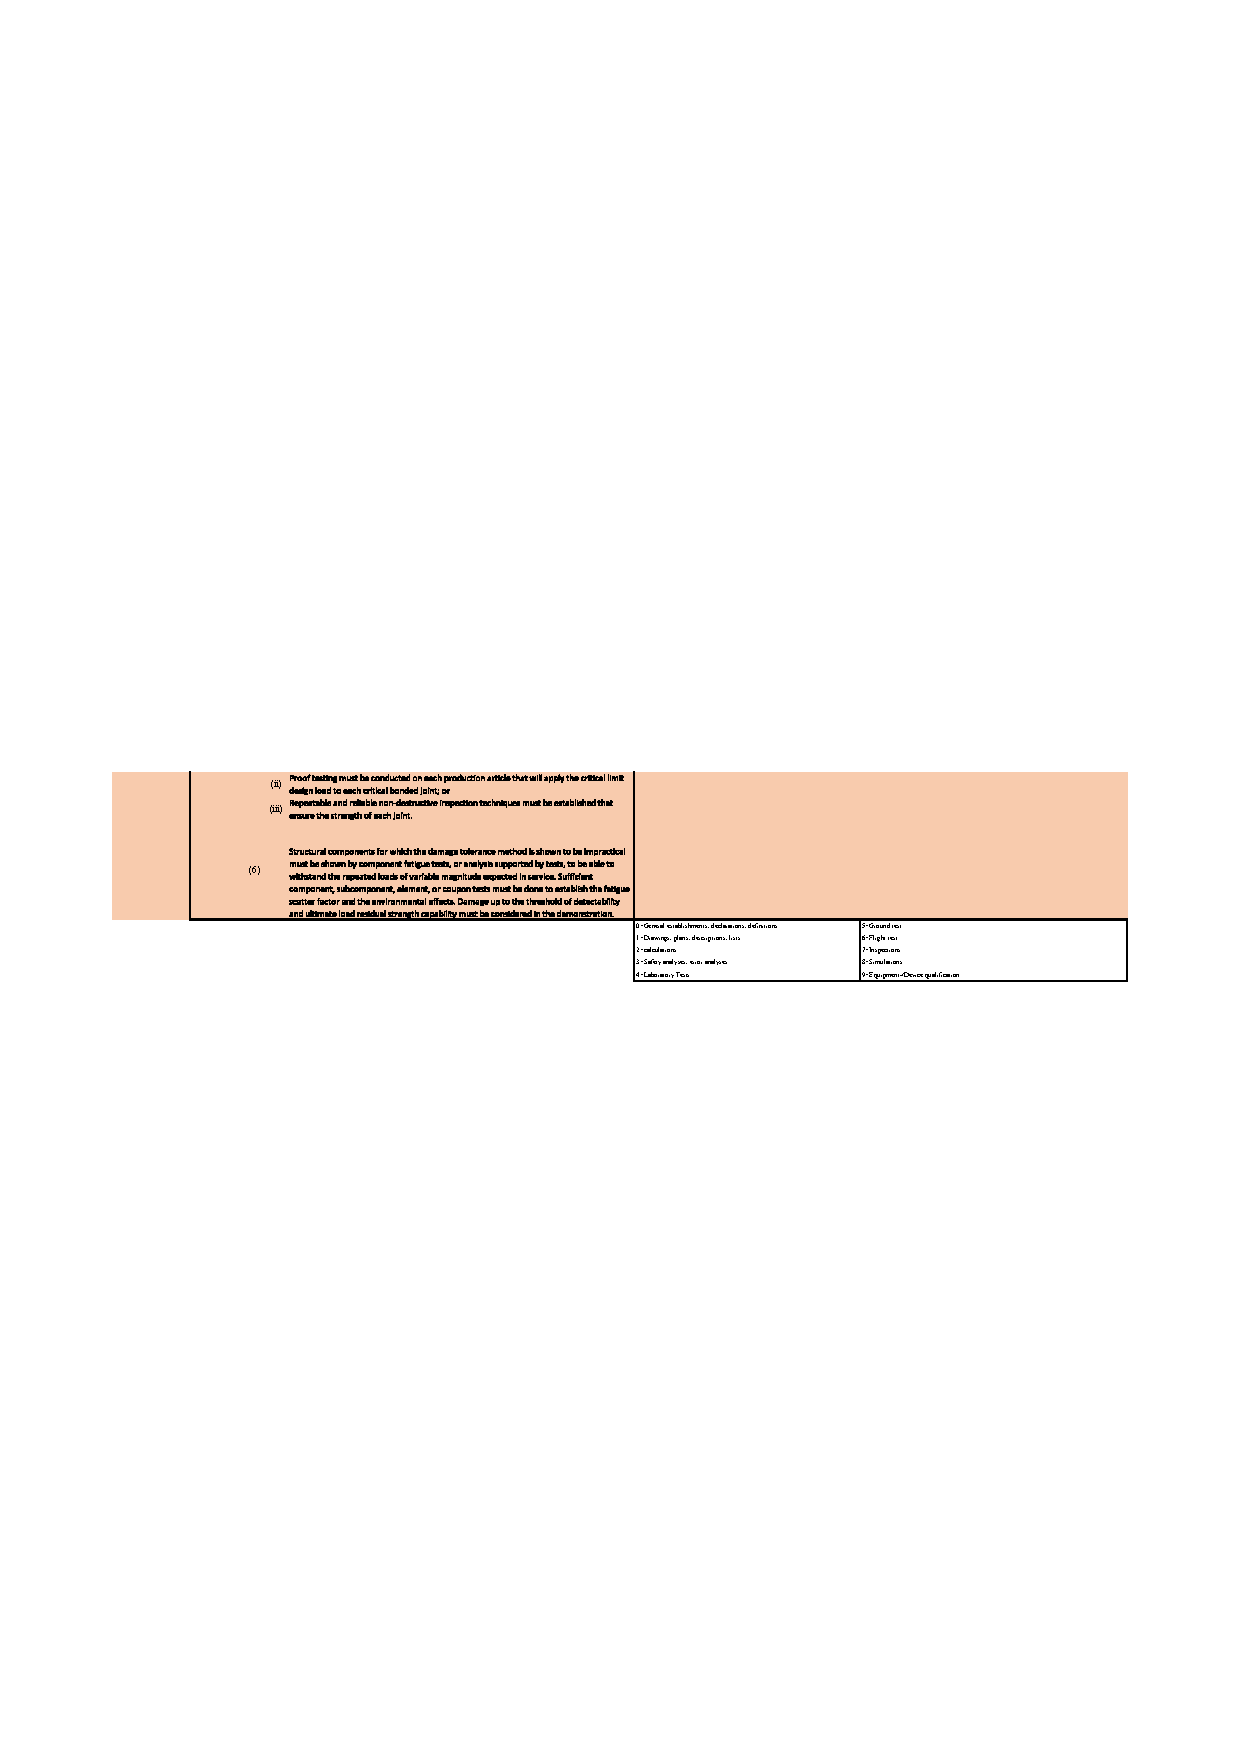
\includegraphics[width=0.9\textwidth]{bilder/Tabellen/MPP_Konstruktion_11.pdf}
\caption{Musterprüfplan} 
\label{tab:Musterprüfplan}
\end{table}

%\clearpage

\section{}\label{}




\end{document}